\documentclass[
	a4paper,
	twoside,
	11pt,
	numbers=noenddot, 				% No dot after numbers for chapters, sections, etc.
	cleardoublepage=empty, 			% Left plain page before chapters
	%DIV=15,            			% Adjust this value for more/less text on pages
	BCOR=5mm 						% Binding correction
]{scrbook}

%%%%%%%%%%%%%%%%%%%%%%%%%%%%%%
%%%%%%%%%% Preamble %%%%%%%%%%
%%%%%%%%%%%%%%%%%%%%%%%%%%%%%%

% Kopf- und Fusszeile
\usepackage[manualmark]{scrpage2} 	% Package scrpage2 erlaubt es die Kopf- und Fußzeile zu gestalten. Optionen sind automark oder manualmark
\pagestyle{scrplain}				% Nur Seitenzahl in Fußzeile. Sonst bleibt Kopf- und Fußzeile leer. Mit "headings" wird Kopf- und Fußzeile eingebunden
\ofoot[]{} 							% Seitenzahl am Rand wird nur gesetzt wenn \pagemark eingefügt wird. Wenn es leer bleibt wird nichts geschrieben
\cfoot[\pagemark]{\pagemark} 		% Seitenzahlen in der Seitenmitte, wenn \pagemark eingefügt. Ansonsten keine Seite

\setlength{\parindent}{0pt} 		% Indent ist set to the given value

% Sprache
\usepackage[english, german]{babel}
\usepackage{verbatim} 				% Text in the env "comment" is interpreted as a comment

% mathematical packages
\usepackage{amsmath}
\usepackage{mathtools}
\usepackage{amssymb}
\usepackage{physics} 				% Usefull package for physical and mathematical formulas. Package-documentation: http://ftp.fau.de/ctan/macros/latex/contrib/physics/physics.pdf
%\usepackage{bbold}					% to write the unit element like lettes with \mathbb
\usepackage{dsfont}					% to write the unit element with \mathds, see: http://milde.users.sourceforge.net/LUCR/Math/mathpackages/dsfont-symbols.pdf

% package for including graphics
\usepackage{graphicx}
\usepackage{subfigure} 				% Package for setting two graphics side by side
\usepackage{epstopdf} 				% Convert eps-files to pdf-files
\graphicspath{{figures/}} 			% Path to all figures used in this document

\usepackage{bm}						% Make the argument bold
\usepackage{xcolor}					% Package for changing he color of letters, numbers and other things 
\usepackage{float}					% Improve interface of floating objects

\usepackage{enumitem} 				% change the level in enumerate-envirement

\usepackage[draft]{todonotes}   	% draft: notes showed, disable: not showed

% feynman and wick stuff
\usepackage{simplewick}				% drawing wick contractions above or below a set of operators. See http://ftp.riken.jp/tex-archive/macros/latex/contrib/simplewick/simplewick.pdf

% bibiography package and stylesetting
\usepackage[
	backend = biber, 
	bibencoding = utf8,
	style = alphabetic, 
	sorting = none, 
	autocite = plain, 
	language = autobib,
]{biblatex} 
\addbibresource{bibliography/masterthesis.bib}
\usepackage{csquotes}
\usepackage[colorlinks=true, linkcolor=black, citecolor=black, urlcolor=blue]{hyperref}
%\usepackage{hyperref}
%\usepackage[figure,table]{hypcap}               % to correct a problem with hyperref
%\hypersetup{
%	pdftitle = {},
%	pdfsubject = {},
%	pdfauthor = {},
%	pdfkeywords = {},
%	pdfcreator = {},
%	pdfproducer = {LaTeX with hyperref},
%	colorlinks = true,
%	linkcolor = blue,
%	anchorcolor = blue,
%	citecolor = blue,
%	filecolor = red,
%	menucolor = red,
%	pagecolor = red,
%	urlcolor  = blue,
%	breaklinks = true,
%	pdfstartview = FitV,
%	pdfhighlight = /I,
%	pdfpagelayout = OneColumn,
%	hypertexnames=true
%}


%%%%%%%%%%%%%%%%%%%%%%%%%%%%%%%%%%%%%%%%%
%%%%%%%%%% self-defined macros %%%%%%%%%%
%%%%%%%%%%%%%%%%%%%%%%%%%%%%%%%%%%%%%%%%%

\newcommand{\mt}[1]{\mathrm{#1}} %%% text in math-mode get normal like you aren't in math-mode

%%% braket notation in the hilbertspace of operators (Liouville space) %%%

\newcommand{\oket}[1]{\big|{#1}\big)} % ket in operator space with automatic sizing
\newcommand{\toket}[1]{|\mt{#1})} % ket in operator space for writing inside normal text

\newcommand{\obra}[1]{\big({#1}\big|} % bra in operator space with automatic sizing
\newcommand{\tobra}[1]{(\mt{#1}|} % bra in operator space for writing inside normal text

\newcommand{\obraket}[2]{\big({#1}\big|{#2}\big)} % braket in operator space with automatic sizing
\newcommand{\tobraket}[2]{({#1}|{#2})} % braket in operator space for writing inside normal text

\newcommand{\odyad}[2]{\oket{#1}\obra{#2}} % dyad in operator space with autometic sizing
\newcommand{\tdyad}[2]{\toket{#1}\tobra{#2}} % dyad in operator space for writing inside normal text

\newcommand{\ie}{i.\,e.}

%\newcommand{\ev}[1]{\left\langle{#1}\right\rangle} 											% expactation value
%\newcommand{\erwartungswert}[3]{\left\langle {#1}\right|{#2}\left|{#3}\right\rangle} 		% ausführlicher erwartungswert mit zuständen
%\newcommand{\kom}[2]{\Big[{#1},{#2}\Big]} 													% commutator
%\newcommand{\antikom}[2]{\Big\{{#1},{#2}\Big\}} 											% anticommutator
%\newcommand{\integral}[4]{\int\limits_{{#1}}^{{#2}}{#3}\ {#4}} 								% integral: #1->lower limit; #2->upper limit; #3->differential operator; #4->integrand
%\newcommand{\scalarproduct}[2]{\left({#1}|{#2}\right)} 										% scalar product super operator
%\newcommand{\opnorm}[1]{\left({#1}|{#1}\right)} 											% norm super operator
%\newcommand{\evso}[3]{\left({#1}\right|{#2}\left|{#3}\right)} 								% expactation value super operator
%\newcommand{\projectionoperator}[2]{\frac{\left|{#1}\right)\left({#2}\right|}{\opnorm{#2}}} % projectionoperator super operator
%\newcommand{\opket}[1]{\left|{#1}\right)} 													% operator ket
%\newcommand{\opbra}[1]{\left({#1}\right|} 													% operator bra
%\newcommand{\trace}[1]{\mathrm{Tr}\left\{{#1}\right\}} 										% trace
\newcommand{\green}[2]{\big\langle\big\langle{#1};{#2}\big\rangle\big\rangle} 				% Definition of Green-function with angle brackets
%\newcommand{\totalDif}[1]{\frac{\mathrm{d}}{\mathrm{d}{#1}}} 								% totale differentiation
%\newcommand{\partialDif}[1]{\frac{\partial}{\partial{#1}}} 									% partielle differentiation
%\newcommand{\longkom}[2]{\Big[{#1},\vphantom{\Big]}\notag\\\vphantom{\Big[}&{#2}\Big]} 		% commutator with linebreak between #1 und #2
%\newcommand{\longev}[2]{\Big\langle{#1}\\ &{#2}\Big\rangle}									% expectation value with linebreak between #1 and #2

% Vectors and matricies
%\newcommand{\bvec}[1]{\textbf{#1}} 															% vector bold letter
%\newcommand{\oneTwoVec}[2]{\begin{pmatrix}#1 & #2\end{pmatrix}} 							% two componand row vector
%\newcommand{\twoOneVec}[2]{\begin{pmatrix}#1\\#2\end{pmatrix}} 								% two componand column vector
%\newcommand{\twoTwoMatrix}[4]{\begin{pmatrix}#1 & #2\\#3 & #4\end{pmatrix}} 				% 2x2 matrix

% Fourier transformation
%\newcommand{\fouriertrafo}[4]{\int \frac{\mathrm{d}^{#4}{#3}}{(2\pi)^{#4}}\, {#1}({#3},\tau) e^{#2}} % Fouriertrafo into momentum space (#1: function; #2: argument of e; #3: momentum letter; #4: dimension)

% definition of mathematical functions
\DeclareMathOperator{\sign}{sign}
%\DeclareMathOperator{\Real}{Re}
%\DeclareMathOperator{\Imag}{Im}

%%%%%%%%%%%%%%%%%%%%%%%%%%%%
%%%%%%%%%% Layout %%%%%%%%%%
%%%%%%%%%%%%%%%%%%%%%%%%%%%%








%%%%%%%%%%%%%%%%%%%%%%%%%%%%%%%%%%%%%%%%%%%%%%%
%%%%%%%%%% Beginning of the document %%%%%%%%%%
%%%%%%%%%%%%%%%%%%%%%%%%%%%%%%%%%%%%%%%%%%%%%%%

\begin{document}

\pagestyle{empty}					% no pagestyle -> no heading, no numbering
\selectlanguage{german}				% document language set to german

%%% Your personal titlepage in german
%%% Can be used for diplomathesises
%%%
%%% adjust all the red colored text and remove the color tags

\begin{titlepage}
  \rmfamily
  \begin{center}
    { \Large
      \hrule
      \vspace{1em}
      \begin{center}

        \begin{minipage}[hbt]{4cm}
          \centering
          
\includegraphics[draft=false, width=3cm]{logos/KITlogo_transparent.eps}
        \end{minipage}
        \begin{minipage}[hbt]{11cm}
          Fakult"at f"ur Physik

          Institut f"ur Theorie der Kondensierten Materie
        \end{minipage}
      \end{center}
      \vspace{1em}
      \hrule 
    } 
    \vspace*{\stretch{11}}
    { 
      \LARGE\bfseries
      Quantentransport in Spindichtesystemen mit dem Memory-Matrix-Formalismus\\       
    }
    \vspace*{\stretch{14}}
    {
      %\includegraphics[width=10cm]{Titlepage/cover}\\
    }
    \vspace*{\stretch{8}}
    { \Large
      Masterthesis \\
      \vspace*{\stretch{0.5}}
      von \\
      \vspace*{\stretch{0.5}}
      Martin Lietz\\
    }
    \vspace*{\stretch{2}}
    { \large 
      27.\,Mai\,2017 bis 27.\,Mai\,2018\\
    }
    \vspace*{\stretch{5}}
    { \large
      \begin{tabular}{r@{\hspace{2em}}l}
        Referent:     & Prof.\,Dr.\,J"org Schmalian\\
        Korreferent:  & Prof.\,Dr.\,Alexander Shnirman
      \end{tabular}
    }
  \end{center}
  \vspace*{\stretch{1}}
\end{titlepage}
\cleardoublepage
		% titlepage in german
%%%% Your personal titlepage in german
%%% Can be used for diplomathesises
%%%
%%% adjust all the red colored text and remove the color tags

\begin{titlepage}
  \rmfamily
  \begin{center}
    { \Large
      \hrule
      \vspace{1em}
      \begin{center}

        \begin{minipage}[hbt]{4cm}
          \centering
          
\includegraphics[draft=false, width=3cm]{logos/KITlogo_transparent.eps}
        \end{minipage}
        \begin{minipage}[hbt]{11cm}
          Fakult"at f"ur Physik

           Institut f"ur Theorie der Kondensierten Materie
        \end{minipage}
      \end{center}
      \vspace{1em}
      \hrule 
    } 
    \vspace*{\stretch{11}}
    { 
      \LARGE\bfseries
      Vector $\phi^4$-model in hyperbolic space\\       
    }
    \vspace*{\stretch{14}}
    {
      %\includegraphics[width=10cm]{Titlepage/cover}\\
    }
    \vspace*{\stretch{8}}
    { \Large
      Master's Thesis \\
      \vspace*{\stretch{0.5}}
      by \\
      \vspace*{\stretch{0.5}}
      Alexander Gawrilow\\
    }
    \vspace*{\stretch{2}}
    { \large 
      January 24, 2017 - January 24, 2018\\
    }
    \vspace*{\stretch{5}}
    { \large
      \begin{tabular}{r@{\hspace{2em}}l}
        Advisor:     & Prof.~Dr.~J"org Schmalian\\
        Co-Advisor:  & Prof.~Dr.~Alexander~Shnirman
      \end{tabular}
    }
  \end{center}
  \vspace*{\stretch{1}}
\end{titlepage}
\cleardoublepage
		% titlepage in english

\frontmatter						% activate roman numbering
\pagestyle{plain}

\cleardoublepage
\vspace*{30\baselineskip}
%\hbox to \textwidth{\hrulefill}
\par
\noindent {Ich erkl"are hiermit, dass die Arbeit selbstst\"andig angefertigt, alle benutzten Quellen und Hilfsmittel vollst\"andig und genau angegeben und alles kenntlich gemacht wurde, das aus Arbeiten anderer unver\"andert oder mit Ab\"anderungen entnommen ist.
}
\vspace{1cm}

\noindent
Karlsruhe, den \today{}

\vspace{1cm}

\noindent\dotfill\hspace*{10.0cm}\\
(\textbf{Martin Lietz}) %center name with hspace
		% assertion in german

\selectlanguage{english}			% document language set to english
\cleardoublepage
%
%
\chapter*{Acknowledgment}
%
%
%I would like to express my thanks to my advisor J\"org Schmalian who encouraged and supported me and gave the right hints at the right time during the last year. 
%His essential input lead to the results presented in this work. 

%Furthermore, I would like to thank Una Karahasanovic for all the discussions and information which became decisive for one topic of this work. 

%Then, I have to thank especially Jian Kang who crucially contributed to the discussion of bond currents and Rafael Fernandes for the fruitful discussions on the general topic. 

%Special thanks to all the colleagues of the condensed matter group at the KIT. Especially to Bhilahari Jeevanesan for all the discussions and help with several problems and to Pablo Schad for finalizing this work. 

%Last but not least, I have to thank my family, my mother and sister and especially Anja for all the support and encouraging words. 
 
		% help from colleagues and friends

\cleardoublepage
\tableofcontents					% table of contents

\pagestyle{scrheadings}				% activate heading and numbering
\mainmatter							% activate	arabic numbering

% includeing chapters
\begingroup
\allowdisplaybreaks
\cleardoublepage
\chapter{Motivation}

%
\cleardoublepage
%
%
%
\chapter{Infinite Conductivity in Translation Invariant Systems}
\label{ch:infinite conductivity}
%
%
%
Ever since Drude published his theory about the electrical conductivity in metals \cite{Drude} at the beginning of the last century it is well known that non-conversation of electron momentum in a system is required for finite electrical conductivity.
In Drude's model the electrons possess a mean scattering time $\tau_{\mt{el}}$, which represent the mean time between two scattering events of an electron and a lattice atom.
At each scattering event the electrons transfer momentum to the lattice atoms, which is the reason electron momentum isn't a conserved quantity.
In the case of conserved momentum an applied electrical field, for example, would accelarates the electrons up to an infinite velocity, by what an infinite conductivity is eventuated.

In the following we want to prove the case of infinite conductivity by using the memory-matrix-formalism.
Therfore firstly a short overview over the memory-matrix-formalism is given, where a detailed and explicite deviations follows in chapter \ref{ch: memory matrix formalism}.
Then the electrical conductivity is generally computed for a system with conserved momentum.
%
%
\section{An Overview over the Memory-Matrix-Formalsim}
\label{sec:overview MMF}
%
%
Let us assume a physical dynamical variable $\mt{A}(t)$ in an arbitrary system and an arbitrary pertubation too	.
Our interest is now the time evolution of $\mt{A}(t)$ depending on the pertubation.
Completely general, a physical dynamical variable can be splitted into two parts, a secular one and a non-secular one, which is shown in \cite{Mori}.
The latter represent processes like fluctuations or initial transient processes, which have in common a short lifetime comparing to the secular processes.
The dynamic and time evolution of $\mt{A}(t)$ is therefore dominated by secular processes.

This seperation enables a simple but clever and intelligent geometrical interpretation, where dynamical variables are considered as vectors in a vector space.
Thereby the variables of the unpertubated system represent the basis vectors of this vector space, denoting in the case of the variable $\mt{A}(t)$ as A-axis.
Due to pertubation the direction of the variabel $\mt{A}(t)$ changes with respect to the A-axis.
The projection of $\mt{A}(t)$ onto the A-axis corresponds to the secular part, where the perpendicular component represents accordingly the non-secular parts.

First of all the mathematical framework has to be considered.
In quantum mechanics the Liouville space, also called as operator space, is the respective vector space of the memory-matrix-formalism.
Like the name operator space should supposed the vectors of the Liouville space are operators, which are certainly Hermitian.
The basis of the Liouville space is signified as $\{\toket{\mt{A}_{i}}\}$, where $i = 1,2,3,\dots,n$, and the corresponding dual space basis is denoted as $\{\tobra{\mt{A}_{i}}\}$.
To make the definition of any vector space complete a scalar product is required, where the following one is chosen.
%
\begin{align}
	\obraket{\mt{A}_{i}(t)}{\mt{A}_{j}(t')} = \frac{1}{\beta} \int\limits_{0}^{\beta} \dd{\lambda} \expval{\mt{A}_{i}^{\dag}(t) \mt{A}_{j}(t'+i\lambda)}
	\label{eq:scalar product Liouville space}
\end{align}
%
The normal time evolution $\mt{A}_{i}(t) = e^{i\mt{H}t/\hbar} \mt{A}_{i}(0) e^{-i\mt{H}t/\hbar}$ of an operator should be valid so that $\mt{A}_{i}(i\lambda) = e^{-\lambda\mt{H}} \mt{A}_{i}(0) e^{\lambda\mt{H}}$ can be used.
The choice of the scalar product is determined under the aspect that as a consequence the time evolution of $\mt{A}(t)$ given the most probably path, if secular processes are neglected, see \cite{Mori}.
In quantum mechanics the dynamic of an operator is ususally described by the Heisenberg equation of motion, which is transformed using the dyad product into the Liouville space.
%
\begin{align}
	\oket{\dot{\mt{A}}_{i}(t)} = \frac{i}{\hbar} \oket{\comm{\mt{H}}{\mt{A}_{i}(t)}} = i \mt{L} \oket{\mt{A}_{i}(t)}
	\label{eq:HEM in LS}
\end{align}
%
where the Hermitian Liouville operator, ${\mt{L} = \hbar^{-1} \comm{\mt{H}}{\mt{\bullet}}}$, is introduced, which is defined by acting onto an arbitrary operator.
The formal solution of this equation is given by $\toket{\mt{A}_{i}(t)} = \exp(it\mt{L}) \cdot \toket{\mt{A}_{i}(0)}$, where the time evolution of an operator is therefore given by the Liouville operator.
In reference to the secular part in a pertubated system a projection operator is defined in the Liouville space.
Starting therefore with a set of arbitrary operators $\{\mt{C}_{i}\}$. 
The choice of the operators is different for each investigated problem and unimportant at the moment.
The definition of the projection operator in Liouville space follows directly from the projection operator defined in the usually used Hilbert space in quantum mechanics.
%
\begin{align}
	\mt{P} = \sum\limits_{i,j} \frac{\oket{\mt{C}_{i}(0)} \obra{\mt{C}_{j}(0)}}{\obraket{\mt{C}_{i}(0)}{\mt{C}_{j}(0)}} 
	\label{eq:projection operator}
\end{align}
%
If the projection operator acting on some vector in Liouville space yields the projection onto the subspace spanned by the operator $\mt{C}_{i}$ and thus the operator $\mt{Q} = 1 - \mt{P}$ yields the corresponding part projected out of the subspace.
Further the projection operator is Hermitian and fullfills the two properties $\mt{P}^{2} = \mt{P}$ and $\mt{PQ} = \mt{QP} = 0$.
This completes the required mathematical basis of the memory-matrix formalism.

Correlation functions are the natural approach describing the reaction of a dynamic variable on a pertubation.
In quantum mechanics the correlation function is defined in Kubo's linear response theory as an integral over an expectation value of two operators, where one of them is certainly the investigated operator and the other one is the coupling operator from the pertubation Hamiltonian.
In the Liouville space the correlation function is defined as
%
\begin{align}
	\mathcal{C}_{ij}(t) := \obraket{\mt{A}_{i}(t)}{\mt{A}_{j}(0)} = \frac{1}{\beta} \int\limits_{0}^{\beta} \dd{\lambda} \expval{\mt{A}_{i}^{\dag}(t) \mt{A}_{j}(i\lambda\hbar)},
	\label{eq:correlation function in LS}
\end{align}
%
where in the second step the definition of the scalar product \eqref{eq:scalar product Liouville space} is only used.
Expressing the time evolution of $\mt{A}_{i}(t)$ with the Liouville operator, using the Laplace transformation and a few conversions yield a algebraic matrix equation of the correlation function, which has the form
%
\begin{align}
	\sum\limits_{l} \Big[\omega \delta_{il} - \Omega_{il} + i \Sigma_{il}(\omega)\Big] \mathcal{C}_{lj}(\omega) = \frac{i}{\beta} \chi_{ij}(0),
	\label{eq:algebraic equation correlation function}
\end{align}
%
where the abbreviations 
%
\begin{align}
	\Omega_{il} := i \beta \sum\limits_{k} \obraket{\dot{\mt{A}}_{i}}{\mt{C}_{k}} \chi_{kl}^{-1}(0)
	\qq{and}
	\Sigma_{il}(\omega) := i \beta \sum\limits_{k} \obra{\dot{\mt{A}}_{i}} \mt{Q} \frac{1}{\omega - \mt{QLQ}} \mt{Q} \oket{\dot{\mt{C}}_{k}} \chi_{kl}^{-1}(0)
	\label{eq:Omega&Sigma}
\end{align}
%
are introduced.
Both sums over $l$ and $k$ runs over the set of operators, defined by the projection operator.
Similiarly the indices $i$ and $j$ has to be chosen out of this set of operators, so that \eqref{eq:algebraic equation correlation function} yields $n^{2}$ equations, if $n$ is the number of operators in the set.
Both abbreviations can be combine to a function $M_{il}(\omega) := \Sigma_{il}(\omega) +i \Omega_{il}$, called the memory function.
Thereby $\Sigma_{il}(\omega)$ takes the role of the quantum mechanical self energy and on the other hand $\Omega_{il}$ represents dissipative effects.
In the case of an invariant Hamiltonian with respect to time reversal symmetry and that the operators $\mt{A}_{i}$ and $\mt{C}_{k}$ of the expectation value in $\Omega_{il}$ have same signature under time reversal symmetry $\Omega_{il}$ vanishes.
This assertion is proven in great detail in \ref{subsec: time reversal symmetry}.
Thus the memory function is solely determined by $\Sigma_{il}(\omega)$.

The structur of $\Sigma_{il}(\omega)$ remembers to the one of the Laplace transformed correlation function, comparing equation \eqref{eq: correlation function frequency space}.
Two things are different.
The expectation value is performed with respect to the operators like $\mt{Q}\toket{\dot{\mt{A}}_{i}}$ instead of $\toket{\mt{A}_{i}}$ and on the other hand only the reduced Liouville operator $\mt{QLQ}$ is considered.
The latter projects at the part of the full Liouville operator, which causes the intrinsic fluctuations of the operator $\mt{A}$.
In other words the operator QLQ describes the internal dynamics of all other degrees of freedom of the system, called the "bath", excluded A.
The coupling to the bath is characterizied by the vector $\mt{Q}\toket{\dot{\mt{A}}_{i}}$.
The coupling to the bath is clearly changing the dynamic behaviour of A.
%
%
\section{Electrical Conductivity in a Momentum Conserving System}
\label{sec:conductivity conserved momentum}
%
%
In the following with the aim of the memory-matrix-formalism the electrical conductivity is computed for a system, where momentum is conserved.
Therefore an infinite conductivity is expected due to the fact that electrons does not transfer any momentum to other degrees of freedom.






























%
\cleardoublepage
%
%
%
\chapter{Spin-Fermion-Model}
\label{ch: spin fermion model}
%
%
%
In the following chapter the spin-fermion-model for a metal exhibiting a antiferromagnetic quantum phase transition is introduced as presented in \cite{Abanov&Chubukov&Schmalian}.
Beside fermionic particle-hole-exitetaions in the vicinity of the quantum critical point bosonic spin fluctuations arise in this low energy theory, which enable a attractive interaction between electrons.
This chapter isn't displayed a detailed mathematical or microscopic derivation of the spin-fermion-model, but rather it is based on a qualitative description to justified its form.
For that a shortly overview over quantum phase transitions are established as suggested in \cite{SachdevQCP}.
In particular, we focus one's attention on the arising spin fluctuations, agrue them carry large momenta and introduced the damped spin density propagator and their perodicity.
Further we present the basic concepts of hot-spot theory, which are points on the Fermi surface in 2D emerged since the magnetic Brillouin zone cutting the Fermi surface.
Besides we review explicitly the conservation of momentum and non-conservation of current for the observing Hamiltonian.
For breaking translation symmetry umklapp scattering is introduced and we prove that this is unconserving momentum.
%
%
\section{Spin-Fermion-Model}
\label{sec:spin-fermion-model}
%
%
Many metals exhibit an antiferromagnetic phase transition at a characteristic temperature $\mt{T}_{\mt{N}}$, called N\'eel-temperature.
The random ordered spins of lattice atoms ordering in consequence of thermal fluctuations along one axis, where the nearest neighbors are always aligned in opposite direction.
This temperature can be changed by tuning a certain parameter like pressure or doping, for example.
A schematic and simplified phase diagram is depicted in figure \ref{fig:phase diagram}.
%
\begin{figure}[t]
	\centering
	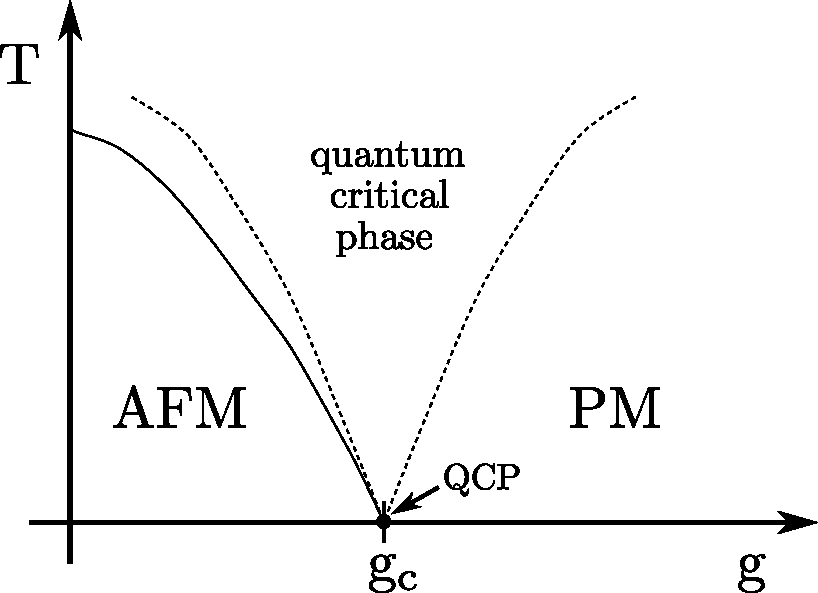
\includegraphics[width=0.7\textwidth]{phase_diagram.pdf}
	\caption{
This figure shows a schematic and simplified phase diagram for metals transition from a paramagnetic (PM) into an antiferrmagnetic (AFM) phase depending on a tunung parameter g.
The phase line of the AFM phase ends decreasing temperature down to $T = 0$ in a quantum critical point (QCP) at $\mt{g} = \mt{g}_{\mt{c}}$.
At this point the phase transition is only caused by quantum fluctuations.
At $T > 0$ thermal fluctuactions more and more dominates the phase transition.
Nevertheless quantum fluctuations influences the physical behaviour in a lagre regime, labeled as quantum critical phase.
	}
	\label{fig:phase diagram}
\end{figure}
%
Decreasing tempearutre the phase line between both magnetic phases reach a certain value for the tuning parameter g at $T = 0$, labeled with $\mt{g}_{\mt{c}}$.
This point is called quantum critical point and in comparsion with the phase transition at finite temperature quantum fluctuations are the origin of this phase transition.

Before starting with a qualitative derivation of the spin-fermion-model a short and rudimentary describtion of quantum phase transition is given.
This overview is required for the analytical discussion of our computation later.
However, the reason for phase transitions is always level crossing between the ground and an excited state.
Due to the fact that level crossing is forbidden a band gap $\Delta$ arises.
This band gap is therefore a characteristic energy scale of the quantum phase transition.
Considering only phase transitions of second order the characteristic energy scale $\Delta$ is proportional to the tuning parameter as
%
\begin{align}
	\Delta \sim \mt{J} |\mt{g} - \mt{g}_{\mt{c}}|^{z \nu},
	\label{eq:energy scale Delta}
\end{align}
%
where $z\nu$ is a critical exponent and J a energy scale of a microscopic coupling \cite{SachdevQCP}.
Beside a characteristic energy scale quantum phase transitions also possesses a characteristic length scale $\xi$, called correlation length, which diverges right at the quantum critical point.
%
\begin{align}
	\xi^{-1} \sim \Lambda |\mt{g} - \mt{g}_{\mt{c}}|^{\nu},
	\label{eq:correlation length xi}
\end{align}
%
where $\nu$ is again a critical exponent and $\Lambda$ an arbitrary inverse length scale like a momentum cut-off, for example.
Inserting \eqref{eq:correlation length xi} in \eqref{eq:energy scale Delta} yields a directly relation between both characteristic quantities.
For finite temperatures, $T > 0$, a second energy scale is given by $k_{\mt{B}} T$, where $k_{\mt{B}}$ is the Botzmann constant.
Comparing both energy scales yields a proportionality between temperatur and correlation length as
%
\begin{align}
	T \sim \xi^{-z}.
	\label{relation temperature and correlation length}
\end{align}
%
Further this explaines the curved conical boundary phase lines of the quantum critical phase in figure \ref{fig:phase diagram}.
In the case of small temperatures the critical exponent $z$ attains the value $z = 2$, so that the phase lines are shaped like a square root.
Increasing temperature the phase boundary lines are linear, since the critical exponent changing to $z = 1$ \cite{Patel&Sachdev}.
Inside this regime the physical behaviour of the metals is determined by quantum fluctions.

Knowing the physical origin of quantum phase transitions the spin-fermion-model can be introduced.
Instead of an microscopic and detailed mathematical describtion we want focus our introduction on qualitative arguments motivating the model.
The spin-fermion-model describes metals in the vicinity of a magnetic quantum critical point considering fermionic quasiparticles and bosonic spin density waves.
Thereby, the propagator is determined by the usual free fermionic Green function.
Spin fluctuations are constituted as collective modes and their propagator is characterized by the dynamical magnetic susceptibility.
%
\begin{align}
	\mathcal{D}_{\mu}(\vb{q}, \omega) = \sum\limits_{\vb{Q}} \frac{1}{(\vb{q}+\vb{Q})^{2} + \xi^{-2} - (\flatfrac{\omega}{v_{\mt{S}}})^{2}},
	\label{eq:undamped spin propagator}
\end{align}
%
where $\mu$ is the spatial direction of the spin density wave, $\xi$ the magnetic correlation length and $v_{\mt{S}}$ the spin wave velocity.
The spin wave velocity is of the same order as the Fermi velocity since spin fluctuations originate due to fermions in the vicinity of the Fermi surface.
Furthermore, the magnetic susceptibility possesses a peak at the momentum vector $\vb{Q} = (\pi, \pi)$.
This implicates a strong coupling interaction between momentum vectors $\vb{k}$ and $\vb{k} + \vb{Q}$.

Phase transitions are always associated by an order parameter equally the investigated antiferromagnetic phase transition, where the local magnetization measured by the spin expectation value $\expval{\mt{S}_{\mu}}$ is the corresponded one.
Similar to the propagator the index $\mu$ indicated the spatial direction.
The order parameter is finite in the antiferromagnetic ordered phase and reaches zero in the paramagnetic disordered phase.
Further, the expectation value of the spin operator is spatially modulated according to $\expval{\mt{S}_{\mu}} \sim e^{i\vb{Q}\vb{R}}$, where $\vb{R}$ is some lattice vector \cite{Weiss}, and therefore the order parameter and equally the propagator are periodical quantities.
In reciprocal space this is reflected in the periodicity  of the magnetic Brillouin zone spanned by the vector $\vb{Q}$.

Our describtion of the antiferromagnetic quantum phase transition in the spin-fermion-model is based on a few fundamental assumptions, comparatively to \cite{Abanov&Chubukov&Schmalian}.
We assume spin fluctuations arise over a large range of the tuning parameter and other low-energy collective degrees of freedom, independent on spin excitations, are neglectable.
Starting by large values of the tuning parameter g, where the metal is in the paramagnetic phase, the physical behaviour is described by Landau's Fermi liquid theory.
Decreasing the tuning parameter and getting closer to the quantum critical point changes the behaviour of the Fermi liquid.
Assuming only one type of fermions the arising collective modes are originated due to permanent interaction between particles and holes.
These bosonic spin excitations determine the physics in the vicinity of the quantum critical point and turning into smooth modes.
Therefore, we assume that only one dominant channel exist for fermion-fermion interaction with energies smaller than an energy cut-off $\Lambda$.
Further we introduce on collective spin mode which containts this interaction.
\todo{Diesen Abschnitt nochmal \"uberarbeiten}
The obtained effective Hamiltonian for the spin fluctuations in the low-energy theory is given by
%
\begin{align}
	\mt{H}_{\Phi} &= 
	 	\int_{\vb{k}}\, \Big[-\frac{\vb{k}^{2}}{2} - \frac{r}{2}\Big] \Phi_{\mu}(\vb{k},\tau) \Phi_{\mu}(-\vb{k},\tau)
		+
		\frac{v_{\mt{S}}^{2}}{2} \pi_{\mu}(\vb{k},\tau) \pi_{\mu}(-\vb{k},\tau)
	\label{eq:Hamiltonian spin fluctuation}
\end{align}
%

In two dimensions the dimensionless coupling constant $\lambda$ is proportional to the inverse magnetic correlation length $\xi$ and diverges at the quantum critical point.



















%
\cleardoublepage
%
%
%
\chapter{The damped propagator of spin density waves}
\label{ch: propagator}
%
%
%
In the present chapter the propagator of spin density waves should be computed up to the first order in pertubation theory.
The main goal of this masterthesis is the determination of the conductivity for the spin fermion model pertubated via umklapp scattering.
These processes are determined by spin density waves, see section \dots \todo{link to umklapp scattering}, why the propagator of them is needed in the calculation of the conductivity.

Firstly the free spin density wave propagtor is computed.
Therefore the equation of motion of Green functions is used. 
An good introduction of this method can be find in every textbook about quantum field theory in many body physics, but the book by Elk and Gasser \cite{Elk&Gasser} is recommended.
Afterwards the damped propagator is calculated using pertubation theory up the first order.
Finally the obtained propagator is transformed into the Matsubara frequency space.
An easy way to do this is using the Kramer-Kronig relations \eqref{eq: Kramer-Kronig relation}.
%
%
\section{The free propagator of spin density waves}
\label{sec: free propagator}
%
%
In \ref{sec: linear response theory} the linear response theory is established and the retarded susceptibility is introduced this way.
A susceptibility describes the dynamical behaviour of an operator dependent on an external pertubation.
This quantity is close related with the Green function of particles which is called propagator.
The only difference is that the operators and the expectation value of the Green function are represented in the Heisenberg picture comparing to the susceptibility, where they are represented with respect to the unpertubated system.

The Green function's equation of motion is easy to get.
Therefore the Green function has only to be derivated with respect to the time.
The amazing result is that the equation of motion is equally for all typs (retarded, advanced and causal) of Green functions.
Only the boundary conditions are different.
The obtained equation of motion and the boundary conditions are transformed in Fourier space.
%
\begin{align}
	\omega \green{\mt{A}}{\mt{B}}_{\omega}^{j} = \expval*{\comm{\mt{A}}{\mt{B}}_{\eta}} + \green{\comm{\mt{A}}{\mt{H}}_{-}}{\mt{B}}_{\omega}^{j}
	\label{eq: algebraic equation chain}
\end{align}
%
where $j$ labels the typ of the Green function (retarded, advanced and causal) and $\omega$ represented that the Green function is in frequency space.
The double angle brackets symbolized the Green function of the operators A and B.
This equation is an algebraic equation or more precisely an infinite algebraic equation chain for the green function.
On the right hand side in general a new more complicated Green function appears.
For this one exists a new equation chain with a more complicted Green function on the right hand side and so on.
In the case of free propagators we are mostly lucky.
The appearing Green function isn't really complicated, so that the initial Green function appears after one or two interativ steps.
Naturally the same procedure can be done for the Green function in Matsubara time representation.
The result is similar to the one above, only the frequency $\omega$ is replaced with the Matsubara frequancy $i\omega_{n}$.
The simplicity and advantage of this method instead of other ones is that only commutator relations of the (field) operators are needed.
Equation \eqref{eq: algebraic equation chain} is all we need to compute the free propagator of spin density waves.

The dynamic of free spin density waves is described by the Hamiltonian $\mt{H}_{\Phi}$, introduced in chapter \ref{ch: spin fermion model}.
Inserting $\mt{H}_{\Phi}$ and bosonic field operators $\Phi_{\mu}$ for A and B in equation \eqref{eq: algebraic equation chain} is the starting point of the following calculation.
Therefore the abbreviation $\green{\Phi_{\mu}}{\Phi_{\mu}}_{\omega}$ is introduced, where the first operator is readed with the momentum argument $\vb{k}+\vb{G}$ and in comparison the second operator is readed with the opposite one, $-\vb{k}-\vb{G}$.
The time argument is equal in both cases, why it is dropped.
%
\begin{align}
	\omega \green{\Phi_{\mu}}{\Phi_{\mu}}_{\omega} &= 
		\expval{\comm{\Phi_{\mu}(\vb{k}+\vb{G})}{\Phi_{\mu}(-\vb{k}-\vb{G})}}
		+
		\green{\comm{\Phi_{\mu}(\vb{k}+\vb{G})}{\mt{H}_{\Phi}}}{\Phi_{\mu}}_{\omega}
		\label{eq: equation chain SDW}
\end{align}
%

The bosonic commutator relations are given in equation (\dots\todo{link zu bosonischen Vertauschungsrelationen}).
The only non-vanishing commutator relation is that between the bosonic field operator and the corresponding canonical momentum operator.
Therefore on the right hand side of \eqref{eq: equation chain SDW} the inhomogeneity is vanished.
Computing the Green function on the same side the Hamiltonian $\mt{H}_{\Phi}$ in equation \dots \todo{link zu $H_{\Phi}$} is used.
The commutator is given by
%
\begin{align}
	\comm{\Phi_{\mu}(\vb{k}+\vb{G},t)}{\mt{H}_{\Phi}} &= 
		-\frac{1}{2\epsilon} 
		\sum\limits_{\vb{P}} 
		\int_{\vb{p}}
		\comm{\Phi_{\mu}(\vb{k}+\vb{G},t)}{\pi_{\lambda}(\vb{p}+\vb{P},t) \pi_{\lambda}(-\vb{p}-\vb{P},t)}
	\notag \\
	\Leftrightarrow\ \comm{\Phi_{\mu}(\vb{k}+\vb{G},t)}{\mt{H}_{\Phi}} &= 
		-\frac{1}{2\epsilon} 
		\sum\limits_{\vb{P}} 
		\int_{\vb{p}} \bigg[
			\pi_{\lambda}(\vb{p}+\vb{P},t) \comm{\Phi_{\mu}(\vb{k}+\vb{G},t)}{\pi_{\lambda}(-\vb{p}-\vb{P},t)}
			\notag \\& \hspace{2cm}
			+
			\comm{\Phi_{\mu}(\vb{k}+\vb{G},t)}{\pi_{\lambda}(\vb{p}+\vb{P},t)} \pi_{\lambda}(-\vb{p}-\vb{P},t)
		\bigg]
	\notag \\
	\Leftrightarrow\ \comm{\Phi_{\mu}(\vb{k}+\vb{G},t)}{\mt{H}_{\Phi}} &= 
		-\frac{i}{\epsilon} \pi_{\mu}(\vb{k}+\vb{G},t)
\end{align}
%
where the sum over $\lambda$ is implied at the beginning.
Inserting the obtained result of the commutator in equation \eqref{eq: equation chain SDW} yields the relationship between the initial and the new Green function.
%
\begin{align}
	\omega \green{\Phi_{\mu}}{\Phi_{\mu}}_{\omega} &= 
		-\frac{i}{\epsilon} \green{\pi_{\mu}}{\Phi_{\mu}}_{\omega}
	\label{eq: first item of the chain}
\end{align}
%
Equally to the initial Green function an algebraic equation chain is established for the new Green function.
%
\begin{align}
	\omega \green{\pi_{\mu}}{\Phi_{\mu}}_{\omega} &= 
		\expval{\comm{\pi_{\mu}(\vb{k}+\vb{G},t)}{\Phi_{\lambda}(-\vb{k}-\vb{G},t)}}
		+
		\green{\comm{\pi_{\mu}(\vb{k}+\vb{G},t)}{\mt{H}_{\Phi}}}{\Phi_{\mu}}_{\omega}
\end{align}
%
Like above the same things are to do.
The inhomogeneity is given by the commutator relations \dots \todo{link to commutator relations}.
In comparison to the case above the commutator dosen't vanish this time but it yields $-i$.
For the Green function on the right hand side the commutator has to be calculated again, which yields $\comm{\pi_{\mu}(\vb{k}+\vb{G},t)}{\mt{H}_{\Phi}} = i \big((\vb{k}+\vb{G})^{2} + r_{0}\big) \Phi_{\mu}(\vb{k}+\vb{G},t)$.
In total we obtain the relation
%
\begin{align}
	\omega \green{\pi_{\mu}}{\Phi_{\mu}}_{\omega} = 
		-i + i\Big((\vb{k}+\vb{G})^{2} + r_{0} \Big) \green{\Phi_{\mu}}{\Phi_{\mu}}_{\omega}.
		\label{eq: second item of the chain}
\end{align}
%
Again on the right hand side a new Green function appears.
This time the new Green function is well known, it's the initial one.
Both equations \eqref{eq: first item of the chain} and \eqref{eq: second item of the chain} are an equation system, where the Green function $\green{\pi_{\mu}}{\Phi_{\mu}}$ can be eliminated.
The easiest way doing this is to multiply equation \eqref{eq: first item of the chain} with $\omega$ and inserting \eqref{eq: second item of the chain} in the obtained relation.
%
\begin{align}
	\mathcal{D}_{\mu}^{(0)}(\vb{k},\omega) := \green{\Phi_{\mu}}{\Phi_{\mu}}_{\omega} = \sum\limits_{\vb{G}} \frac{1}{(\vb{k}+\vb{G})^{2} + r_{0} - \xi^{-2}}
	\label{eq: free spin density wave propagator}
\end{align}
%
where the inverse squared correlation length $\xi^{-2} = \epsilon \omega^{2}$ is introduced.
The free propagator exhibits a periodicity with respect to the first Brillouin zone.
This condition is used in the calculation of the static conductivity in chapter \ref{ch: calculation}. 
\todo{say a little bit more about that}
%
%
\section{The damped spin density wave propagator}
\label{sec: damped propagator}
%
%
In the previous section the free propagator of spin density waves is computed.
Beside the free dynamics the spin fermion model considers an interaction between electrons living on different Fermi surfaces, where the interaction is originated by spin density waves.
On that reason the propagation of the spin density waves is damped.
The damping should be considered in the propagator via doing pertubation theory.

Because the damping is originated by the interaction between electrons the free electron propagator is also needed in the following calculation.
The propagator can be calculated in the same way as the  one for free spin density waves.
This handwork shouldn't be done here explicitly.
The free electron propagator is given by
%
\begin{align}
	 \mathcal{G}_{\alpha}^{(0)}(\vb{k},\omega) := \green{\Psi_{\alpha}}{\Psi_{\alpha}^{\dag}}_{\omega} = \sum\limits_{\vb{G}} \frac{1}{\omega - \epsilon_{\alpha}(\vb{k}+\vb{G})}, 
	 \label{eq: free electron propagator}
\end{align}
%
where $\alpha = \mt{a,b}$ denotes the Fermi surface of the respective electrons.
The damped spin density wave propagator is computed using the usually method of pertubation theory in quantum field theory.
The full spin density wave propagator is given by
%
\begin{align}
	\mathcal{D}_{\mu}(\vb{k}, t-t') = -i \expval{\mathcal{T}_{t} \mt{U}(\infty, -\infty) \Phi_{\mu}(\vb{k}+\vb{G},t) \Phi_{\mu}(-\vb{k}-\vb{G},t')}_{0}^{\mt{con}}
	\label{eq: full spin density wave propagator}
\end{align}
%
where $\mathcal{T}_{t}$ is the time ordering operator, which orders all contained operators of there right time order.
The index $0$ denotes that the expectation value is performed with respect to the unpertubated Hamiltonian.
The interaction is only incorporated through the time evolution operator $\mt{U}$ which is given by
%
\begin{align}
	\mt{U}(t,t') = \exp\bigg(-i\int_{t'}^{t} \dd{t_{1}} \mt{H}_{\mt{int}}(t_{1})\bigg).
	\label{eq: time evolution operator}
\end{align}
%
The second index "con" at the expectation value denotes that only connected diagrams are considered.
In the so called link cluster theorem it is proven that all disconnected diagrams are canceled with the vacuum diagrams, see \cite{Nolting} for it.
All these connected diagrams can be simplified a little bit more.
There exist diagrams which are contained only diagrams of a lower order in a specific way.
It is possible to build these diagrams by multipling diagrams of lower orders.
Therefore a new object $\Pi$ is introduced, called self energy, which contains all irreducible connected diagrams.
The self energy offers the oppertunity to write the full Green function as a Dyson equation.
%
\begin{align}
	\mathcal{D}_{\mu} = \mathcal{D}_{\mu}^{(0)} + \mathcal{D}_{\mu}^{(0)} \Pi_{\mu} \mathcal{D}_{\mu}
	\qquad \Rightarrow\ \qquad
	\mathcal{D}_{\mu} = \frac{1}{\big(\mathcal{D}_{\mu}^{(0)}\big)^{-1} - \Pi_{\mu}}
	\label{eq: Dyson equation}
\end{align}
%
In general the self energy is a complex quantity.
Splitting her in a real and imaginary part the real part of its is a correction to the energy and the imaginary part is interpreted as a life time.
A finite life time correspondes to a damped particle.
The goal of the following calculation is to compute the imaginary part of the self energy.
Getting a feeling how the self energy looks in diagrammatic language the full propagator in \eqref{eq: full spin density wave propagator} is investigated.

The time evolution operator is expanded up to the second order.
The zeroth order yields the free propagator which is calculated in the previous section.
Further the first order vanishes.
The interaction Hamiltonian $H_{\Psi\Phi}$ contains one bosonic field operator and therefore combining with the two other bosonic operators this yields an expectation value of three bosonic operators.
Wick's theorem says that the expectation value of an odd number of operators is always zero.
The reason is that it's impossible to get an term where only contractions are contained.
Having an odd number of operators a normal product exist in every term.
Taking the equillibrium expectation value of a normal product, it's zero by definition.

The first not vanishing contribution appears at the second order, because the interaction Hamiltonian $H_{\Psi\Phi}$ contributes twice, thus the number of operators is even in both cases, fermionic and bosonic.
In the fermonic case four expectation values appear, where those ones have a little bit different structure like the usually known ones of fermionic operators.
The feature of them is that two fermionic operators are connected by a Pauli matrix, which prohibit the use of Wick's theorem or any rearrange of the operators.
The expectation values has the special form
%
\begin{align}
	\expval{\mathcal{T}_{t}\ \Psi_{\alpha}^{\dag}(\vb{p}_{4},t_{2}) \cdot \sigma_{\lambda'} \cdot \Psi_{\beta}(\vb{p}_{3},t_{2}) \cdot \Psi_{\gamma}^{\dag}(\vb{p}_{2},t_{1}) \cdot \sigma_{\lambda} \cdot \Psi_{\beta}(\vb{p}_{1},t_{1})}_{0},
	\label{eq: structure of fermionic expval}
\end{align}
%
where $\alpha,\beta,\gamma,\delta \in \{\mt{a},\mt{b}\}$ with the property that always two greek letters have to be an "a" and the other two ones a "b".
Fierz identity offers the oppertunity to eliminate the Pauli matricies.
With the aid of Fierz identity a product of the components of two Pauli matricies can be rewriten as a relation of Kronecker symbols.
%
\begin{align}
	\sum\limits_{\mu = 1}^{3} \sigma_{ij}^{\mu} \sigma_{kl}^{\mu} = 2 \delta_{il} \delta_{jk} - \delta_{ij} \delta_{kl}
	\label{eq: Fierz identity}
\end{align}
%
Acting Fierz identity the product of field operators and Pauli matrix has to be writen in component representation.
Then the identity can be use without any doubt and the Kronecker symbols allows us to rewrite the operators without component representation.
Doing this we have to rivet on the first term in \eqref{eq: Fierz identity}, because the order of the operators is rearranged.
Therefore the operators has to be commuted  with yields a $\delta$-distribution with respect to the momentum, see \eqref{appeq: general expectation value after Fierz identity}.
The exact calculation is done in the appendix \ref{app: Fierz identity}.

Each obtained expectation values contains two operators of a-electrons\footnote{a-electrons denotes electrons living on the Fermi surface labeled with a. In comparison b-electrons are electrons on the Fermi surface labeled with b. Both Fermi surfaces are rotated by $\flatfrac{\pi}{2}$ and shifted by $(\pm\pi,\pm\pi)$ to each other.} and two operators of b-electrons, so that the expectation value can be seperated.
One half of these is constructed in a way that both annihiliation operators are acting with respect to a-electrons, for example.
These kinds of expectation values are surely zero.
The other half is "normaly" constructed so that one annihiliation and creation operator is acting with respect to a-electrons.
The same is surely valid for b-electrons. \todo{writing this argument in a better way}

Bringing the remained operators in the order that all annihilaition operators stands on the left side of the creation operators yields a $\delta$-distribution for each commutation, so that in total each term contains two $\delta$-distributions.
The obtained expectation value is shown in equation \eqref{appeq: expectation value of second order correction} in the appendix \ref{app: Fierz identity}.

Inserting equation \eqref{appeq: expectation value of second order correction} for each of the four expectation values two of the four momentum integrals and sums can be performed.
The remaining expression for $\mathcal{D}$ in second order pertubation theory have the form
%
\begin{align}
	\mathcal{D}_{\mu}^{(2)}(\vb{k}, \omega) &= 
		(-i)^{3} \lambda^{2}
		\int\limits_{-\infty}^{\infty} \dd{t_{1}} \dd{t_{2}}
		\sum\limits_{\vb{P}_{1} \vb{P}_{2}} \int_{\vb{p}_{1}} \int_{\vb{p}_{2}}
		\notag \\ &\times		
		\expval{
			\mathcal{T}_{t} 
			\Phi_{\lambda'} (\tilde{\vb{p}}_{2}-\tilde{\vb{p}}_{1},t_{2}) 
			\Phi_{\lambda} (\tilde{\vb{p}}_{1}-\tilde{\vb{p}}_{2},t_{1}) 
			\Phi_{\mu}(\tilde{\vb{k}},t) 
			\Phi_{\mu}(-\tilde{\vb{k}},t')
		}_{0}
		\notag \\
		&\times
		\bigg(
		\expval{\mathcal{T}_{t} \Psi_{\mt{a}}(\tilde{\vb{p}}_{2},t_{1}) \Psi_{\mt{a}}^{\dag}(\tilde{\vb{p}}_{2},t_{2})}_{0}
		\expval{\mathcal{T}_{t} \Psi_{\mt{b}}(\tilde{\vb{p}}_{1},t_{2})	\Psi_{\mt{b}}^{\dag}(\tilde{\vb{p}}_{1},t_{1})}_{0}
		\notag \\
		&+
		\expval{\mathcal{T}_{t}	\Psi_{\mt{b}}(\tilde{\vb{p}}_{2},t_{1}) \Psi_{\mt{b}}^{\dag}(\tilde{\vb{p}}_{2},t_{2})}_{0}
		\expval{\mathcal{T}_{t}	\Psi_{\mt{a}}(\tilde{\vb{p}}_{1},t_{2})	\Psi_{\mt{a}}^{\dag}(\tilde{\vb{p}}_{1},t_{1})}_{0}
		\bigg)
\end{align}
%
where the abbreviation $\tilde{\vb{k}} = \vb{k}+\vb{G}$ and $\tilde{\vb{p}}_{i} = \vb{p}_{i} + \vb{P}_{i}$ with $i=1,2$ is introduced.
In the case of the bosonic expectation value the usually used Wick theorem is utilized.
Wick's theorem yields three possibile contractions in the corresponding case, where one of these isn't contributed, because it's yielded disconnected diagrams.
The remaining two contractions generate four diagrams in total, which are depicted in figure \ref{fig: all contained bubble diagrams}.
These diagrams differentiate only in two points.

%
\begin{figure}[t]
	\centering
	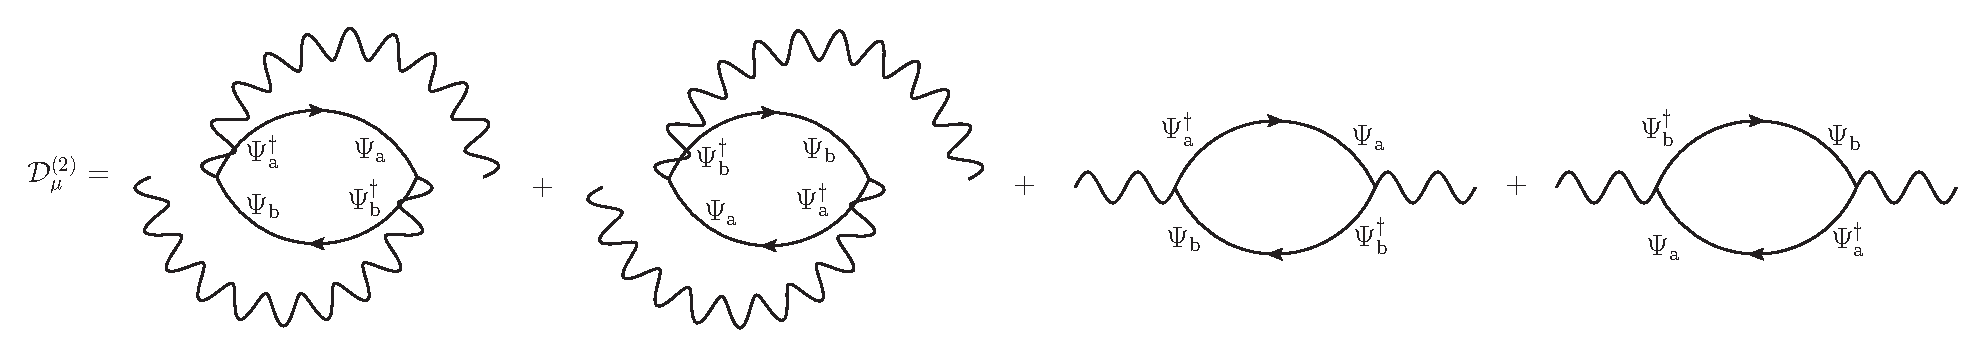
\includegraphics[width=\textwidth]{all_contained_bubble_diagrams.eps}
	\caption{caption}
	\label{fig: all contained bubble diagrams}
\end{figure}
%
On the one hand the acting point of the bosonic lines is changed comparing the first two and last two diagrams.
On the other hand the direction of the electronic lines is interchanged between the first two diagrams and in equal measure for the last two diagrams.
For example, in the first diagram an a-electron is annihiliated and a b-electron is created at $t_{1}$.
Comparing the second diagram, where an a-electron is created and a b-electron is annihilated at $t_{1}$.
All four diagrams are closly connected with each other, because all diagrams can be generated out of one diagram by interchanging the acting point of the bosonic lines or the direction of the fermionic lines.
Therefore all four diagrams yield the same contribution, where it is enough to compute one of them and multiply by four.
%
\begin{align}
	\mathcal{D}_{\mu}^{(2)}(\vb{k}, t-t') &= 
		4i \lambda^{2}
		\int\limits_{-\infty}^{\infty} \dd{t_{1}} \dd{t_{2}}
		\sum\limits_{\vb{P}} \int_{\vb{p}}
		\notag \\ &\times
		\expval{\mathcal{T}_{t} \Phi_{\mu} (\tilde{\vb{k}},t_{2}) \Phi_{\mu}(-\tilde{\vb{k}},t')}_{0}	
		\expval{\mathcal{T}_{t} \Phi_{\mu} (-\tilde{\vb{k}},t_{1}) \Phi_{\mu}(\tilde{\vb{k}},t)}_{0}
		\notag \\ &\times
		\expval{\mathcal{T}_{t} \Psi_{\mt{a}}(\tilde{\vb{p}}-\tilde{\vb{k}},t_{1}) \Psi_{\mt{a}}^{\dag}(\tilde{\vb{p}}-\tilde{\vb{k}},t_{2})}_{0}
		\expval{\mathcal{T}_{t} \Psi_{\mt{b}}(\tilde{\vb{p}},t_{2}) \Psi_{\mt{b}}^{\dag}(\tilde{\vb{p}},t_{1})}_{0}
		\label{eq: spin density wave propagator second order correction}
\end{align}
%
where the momentums $\vb{p}_{1}$ and $\vb{P}_{1}$ are relabeled with $\vb{p}$ and $\vb{P}$, respectivily.
Accordingly we write $\tilde{\vb{p}}$ instead of $\tilde{\vb{p}}_{1}$.
In comparison to the Dyson equation \eqref{eq: Dyson equation} the fermionic bubble is identified with the self energy $\Pi_{\mu}$, where the bubble diagram surely only represented the zeroth order of the self energy.
The self energy in zeroth order is therefore given by
%
\begin{align}
	\Pi_{\mu}^{(0)}(\vb{k}, \omega) = 
		i 
		\sum\limits_{\vb{P}}
		\int\limits_{|p| \leq |p_{\mt{F}}} \frac{\dd[2]{\vb{p}}}{(2\pi)^{2}} 
		\int\limits_{-\infty}^{\infty} \frac{\dd{\epsilon}}{2\pi}\,
		\mathcal{G}_{\mt{a}}^{(0)}(\vb{p}+\frac{\vb{k}}{2}, \epsilon+\frac{\omega}{2})
		\mathcal{G}_{\mt{b}}^{(0)}(\vb{p}-\frac{\vb{k}}{2}, \epsilon-\frac{\omega}{2}).
\end{align}
%
In comparison to equation \eqref{eq: spin density wave propagator second order correction} the self energy is represented in frequency space.
Further the outer momentum and frequency is shifted by the half of itself, so that both arguments of the fermionic propagators are symmetricly, which is depicted in figure \ref{fig: bubble diagram}.
%
\begin{figure}[t]
	\centering
	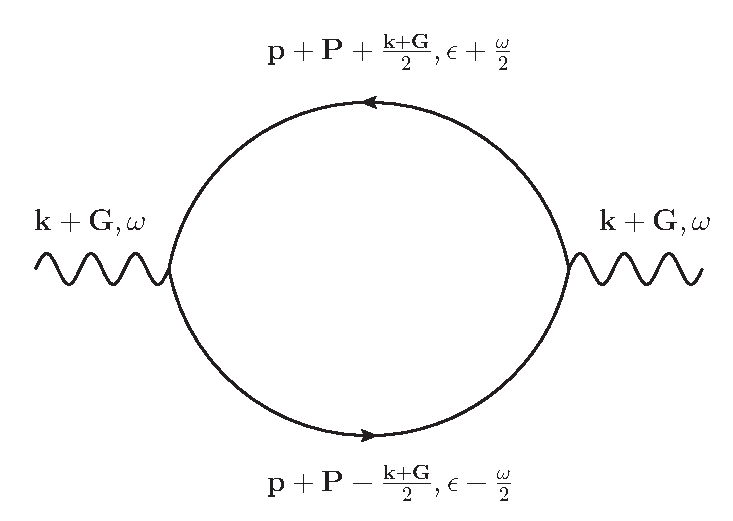
\includegraphics[width=0.5\textwidth]{bubble_diagram.eps}
	\caption{caption}
	\label{fig: bubble diagram}
\end{figure}
%
How we see in equation \eqref{eq: free electron propagator} the free electron propagator contains the dispersion relation $\epsilon_{\alpha}(\vb{p}+\vb{P})$ of the respective electrons.
In our considered spin fermion model only electrons near the Fermi surface interacte with each other interfered by spin density waves, which means that the momentum and energy transfer is small.
Under this condition the dispersion relation can be expanded near the Fermi surface.
%
\begin{align}
	\epsilon_{\mt{a}}(\vb{p} + \vb{P} + \frac{\vb{k} + \vb{G}}{2}) &= 
		\frac{\big(p_{x} + P_{x} + \frac{k_{x} + G_{x}}{2}\big)^{2}}{2m_{1}} 
		+ 
		\frac{\big(p_{y} + P_{y} + \frac{k_{y} + G_{y}}{2}\big)^{2}}{2m_{2}} 
		\notag \\ 
	\Leftrightarrow\ \epsilon_{\mt{a}}(\vb{p} + \vb{P} + \frac{\vb{k} + \vb{G}}{2}) &=
		\frac{(p_{x} + P_{x})^{2}}{2m_{1}} + \frac{1}{2} \frac{p_{x}+P_{x}}{m_{1}}(k_{x}+G_{x}) + \frac{(k_{x}+G_{x})^{2}}{8m_{1}}
		\notag \\ &+
		\frac{(p_{y} + P_{y})^{2}}{2m_{2}} + \frac{1}{2} \frac{p_{y}+P_{y}}{m_{2}}(k_{y}+G_{y}) + \frac{(k_{y}+G_{y})^{2}}{8m_{2}}
		\notag \\
	\Leftrightarrow\ \epsilon_{\mt{a}}(\vb{p} + \vb{P} + \frac{\vb{k} + \vb{G}}{2}) &\approx
		\xi_{\mt{a}} + \frac{1}{2} \vb{v}_{\mt{a,F}}(\vb{k} + \vb{G}) + \mu
\end{align} 
%
where the quadratic term with respect to $\vb{k}$ is neglectable, because the bosonic transfered momentum is assumed as small.
Further the velocity $\vb{v}_{a}$ of the a-electrons is introduced, where the elelctron velocity can be approximated with the Fermi velocity of the corresponding Fermi surface, because only electrons near the Fermi surface are considered.
Besides the dispersion relation $\xi_{\mt{a}}$ of the a-electrons is used, which is given by \dots \todo{link zur dispersion im spin fermion model}.
The same procedure is done for the b-electrons.
Finally the normalized momentum vector $\vb{n} = \frac{\vb{p}+\vb{P}}{|\vb{p}+\vb{P}|}$ is introduced.
The Fermi velocity of the a-electrons is then given by $\vb{v}_{\mt{a,F}} = v_{\mt{a,F}} \vb{n}$ for example.
The scalar product between the normalized momentum vector $\vb{n}$ and the bosonic spin density wave vector $\vb{k} + \vb{G}$ is rewriten as his magnitude multiplied with $\cos(\vartheta)$, where $\vartheta$ is the angle between both.

In the investigated spin fermion model the electrons on different Fermi surfaces only interacte on so called hot spots like we have it introduced in chapter \ref{ch: spin fermion model}.
The energy and the magnitudes of the Fermi velocities are equal on the hot spots.
%
\begin{align}
	\xi := \xi_{\mt{a}} = \xi_{\mt{b}} \qquad v_{\mt{F}} := v_{\mt{a,F}} = v_{\mt{b,F}}
\end{align}
%
Consider that the direction of the velocities haven't been equal, otherwise the angle $\vartheta$ is $0$ or $\pi$ and the imaginary part of $\Pi_{\mu}$ is zero.
Using these assumptions the self energy is given by
%
\begin{align}
	\Pi_{\mu}^{(0)}(\vb{k}, \omega) &= 
		i \nu_{\mt{F}}
		\int\limits_{0}^{\pi} \dd{\vartheta}
		\int\limits_{\xi \leq \xi_{\mt{F}}} \dd{\xi}
		\int\limits_{-\infty}^{\infty} \frac{\dd{\epsilon}}{2\pi}
		\notag \\ &\times
		\frac{1}{\epsilon + \frac{\omega}{2} - \xi - \frac{1}{2} v_{\mt{F}} |\vb{k} + \vb{G}| \cos(\vartheta) + i \eta \sign(\epsilon + \frac{\omega}{2})}
		\notag \\ &\times
		\frac{1}{\epsilon - \frac{\omega}{2} - \xi + \frac{1}{2} v_{\mt{F}} |\vb{k} + \vb{G}| \cos(\vartheta) + i \eta \sign(\epsilon - \frac{\omega}{2})},
	\label{eq: self energy before epsilon integration}
\end{align}
%
where the two dimensional momentum integral is firstly transformed in plane polar coordinates and then the $k$-integral is transformed into an energy integral over the density of states.
Because only electrons near the Fermi surface are considered the density of states can be approximated with the constant one $\nu_{\mt{F}} := \nu(\xi_{\mt{F}})$ at the Fermi surface.
The energy integral is certainly limited by the Fermi energy $\xi_{\mt{F}}$.

The further investigation is been starting with the computation of the frequency integral.
Therefore the integral over $\epsilon$ is transformed into a complex contour integral, where the contour $\Gamma$ is chosen in two different ways.
In both case the contour starts along the real axis.
According to the singularities of the integrand the countour is closed in the upper or lower half plane via a semicircle with radius infinity.
In both cases the contribution of the semicircle is zero because the integrand is proportional to $\flatfrac{1}{\epsilon}$.
The non-contributing of the semicircle ensures the equality between the integral along the real axis and the complex contour integral.
The investigated integrand occupies two singularities at
%
\begin{align}
	\epsilon_{1} := \xi - \frac{1}{2}\big(\omega - v_{\mt{F}} |\vb{k} + \vb{G}| \cos(\vartheta)\big) 
	\qq{and}
	\epsilon_{2} := \xi + \frac{1}{2}\big(\omega - v_{\mt{F}} |\vb{k} + \vb{G}| \cos(\vartheta)\big),
\end{align}
%
where both singularities are of first order which allows using Cauchy's integral formula.
According to the signum function in both denominators the poles are located in the upper or lower plane.
So in total there are four different possible constitutions.
On the one hand both singularities can be located in the lower or upper complex plane, which yield in both cases zero.
On the other hand one pole can be in the upper plane and the other one can be in the lower plane, or vice versa.
Equally both constitutions yields the same contribution.
%
\paragraph{1. case:} $\sign(\epsilon + \frac{\omega}{2}) = \sign(\epsilon - \frac{\omega}{2})$\\
%
Both singularities are located in the upper or in the lower complex half plane.
The contour is therefore closed in the upper or lower plane, respectivily, so that both poles are enclosed.
In the first case the winding number is $1$, because the pole is enclosed counterclockwise.
Accordingly the winding number is $-1$ in the second case.
%
\begin{align}
	&\mt{I}_{\omega}^{\mt{e}} := i \oint_{\Gamma} \frac{\dd{\omega}}{2\pi i}\, \frac{1}{\omega - \omega_{1} \mp i\eta} \cdot \frac{1}{\omega - \omega_{2} \mp i\eta}
	\notag \\
	\Leftrightarrow\ &\mt{I}_{\omega}^{\mt{e}} = \pm i \bigg[ \frac{1}{\omega_{2} - \omega_{1}} + \frac{1}{\omega_{1} - \omega_{2}}\bigg] = 0,
\end{align}
%
where the index "e" stands for even and should mean that both poles are located at the same half planes.
%
\paragraph{2. case:} $\sign(\epsilon + \frac{\omega}{2}) \neq \sign(\epsilon - \frac{\omega}{2})$\\
%
The singularities are located in different complex half planes, one in the upper and accordingly the other in the lower half plane.
In both cases it's arbitrary how the contour is closed.
It's only important that one of the two poles is located inside the contour.
In the following computation the contour is closed in the upper half plane, so the winding number is always $1$.
%
\begin{align}
	&\mt{I}_{\omega}^{\mt{o}} := i \oint_{\Gamma} \frac{\dd{\omega}}{2\pi i}\, \frac{1}{\omega - \omega_{1} \mp i\eta} \cdot \frac{1}{\omega - \omega_{2} \pm i\eta}
	\notag \\
	\Leftrightarrow\ &\mt{I}_{\omega}^{\mt{o}} = \frac{\pm i}{\omega_{2} - \omega_{1} \pm i\eta}
\end{align}
%
where the index "o" stands accordingly for odd and should mean that both poles are located in different half planes.

Inserting both singularities $\omega_{1}$ and $\omega_{2}$ causes that the integrand is independent with respect to the energy $\xi$.
The frequency depending signum functions in \eqref{eq: self energy before epsilon integration} is aquivalent to the signum functions $\sign(\xi \pm \frac{1}{2} v_{\mt{F}} |\vb{k} + \vb{G}| \cos(\vartheta))$ in energy representation.
The energy $\xi$ is neglectable because the integrand is independent of $\xi$.
Further the constant factors are also neglectable because them are always positive. 
The case of sign in the integand depends therefore only on the sign of $|\vb{k} + \vb{G}| \cos(\vartheta)$.
Finally the integrals limits has to be set to $\pm \frac{1}{2} v_{\mt{F}} |\vb{k} + \vb{G}| \cos(\vartheta)$.
This follows directly from the location of the poles.
For example if $\omega_{1}$ is in the lower and $\omega_{2}$ is in the upper half plane than $\epsilon + \frac{\omega}{2} > 0$ and $\epsilon - \frac{\omega}{2} < 0$, respectivily.
Transforming both into energy representation the corresponding expressions are $\xi - \frac{1}{2} v_{\mt{F}} |\vb{k} + \vb{G}| \cos(\vartheta) < 0$ and $\xi + \frac{1}{2} v_{\mt{F}} |\vb{k} + \vb{G}| \cos(\vartheta) > 0$, which yields directly the definition interval of $\xi$.
Therefore we obtained 
%
\begin{align}
	\Pi_{\mu}^{(0)}(\vb{k}, \omega) &= 
		i \nu_{\mt{F}}
		\int\limits_{0}^{\pi} \dd{\vartheta} 
		\int\limits_{-\xi_{0}}^{\xi_{0}} \dd{\xi}
		\frac{i \sign(|\vb{k} + \vb{G}| \cos(\vartheta))}{\omega - v_{\mt{F}} |\vb{k} + \vb{G}| \cos(\vartheta) + i\eta \sign(|\vb{k} + \vb{G}| \cos(\vartheta))}
\end{align}
%
for the self energy, where the abbreviation $\xi_{0} = \flatfrac{v_{\mt{F}}|\vb{k}+\vb{G}|\cos(\vartheta)}{2}$ is introduced.
The integration over $\xi$ yields the factor $v_{\mt{F}}|\vb{k}+\vb{G}|\cos(\vartheta)$.
Subsequently the signum function is reexpressed in frequency representation which corresponds to $\sign(\omega)$.

Like it is shown above the damping of the spin density wave occurs of the imaginary part of the self energy, which is the reason why we take the imaginary part of the above expression in the further computation.
%Formally the real part is absorbed into the mass term $r_{0}$.
The imaginary part of the serlf energy is given by
%
\begin{align}
	\Im{\Pi_{\mu}^{(0)}(\vb{k}, \omega)} &= 
		\nu_{\mt{F}} \pi
		\int\limits_{0}^{\pi} \dd{\vartheta}
		v_{\mt{F}} |\vb{k}+\vb{G}| \cos(\vartheta) \delta(\omega - v_{\mt{F}} |\vb{k} + \vb{G}| \cos(\vartheta)),
	\label{eq: imaginary part of self energy before theta integration}
\end{align}
%
where the formula $\frac{1}{x \pm i\eta} = \PV{\frac{1}{x}} \mp i \pi \delta(x)$ is used.
To perform the last remaining intgeral over $\vartheta$ the $\delta$-distribution has to be rewriten.
The argument is a $\vartheta$ depending function with in general infinite zeros.
But in the integrating area, between $0$ and $\pi$, the cosine only have one zero.
The formula
%
\begin{align}
	\delta(g(x)) = \sum\limits_{i=1} \frac{\delta(x-x_{0,i})}{|g'(x_{0,i})|}
\end{align}
%
states how a $\delta$-distribution with a functional argument can be writen as a sum over $\delta$-distributions with zeros of $g(x)$ as arguments.
The prime denotes the derivative with respect to $x$ which has to be evaluated at the corresponding zero $x_{0,i}$.
The argument of the $\delta$-distribution in \eqref{eq: imaginary part of self energy before theta integration} has a single zero at $\vartheta_{0} = \cos[-1](\flatfrac{\omega}{(v_{\mt{F}} |\vb{k} + \vb{G}|)})$.
Thereby the $\delta$-distribution is rewriten as
%
\begin{align}
	&\delta(\omega - v_{\mt{F}} |\vb{k} + \vb{G}| \cos(\vartheta)) = \Big(v_{\mt{F}} |\vb{k} + \vb{G}| \cdot |\sin(\vartheta_{0})|\Big)^{-1} \delta(\vartheta - \vartheta_{0})
	\notag \\
	\Rightarrow\ &\delta(\omega - v_{\mt{F}} |\vb{k} + \vb{G}| \cos(\vartheta)) \approx \Big(v_{\mt{F}} |\vb{k} + \vb{G}|\Big)^{-1} \delta(\vartheta - \vartheta_{0})
\end{align}
%
where in the second line the limit of small frequancies $\omega$ is performed.
This is valid because of our investigated low energy theory.
In other words the interaction is assumed as small and thereby the frequency and momentum transfer is small too.
Now the integration over $\vartheta$ can be performed easily.
The imaginary part of the self energy is given by
%
\begin{align}
	\Im{\Pi_{\mu}^{(0)}(\vb{k}, \omega)} &= \frac{\nu_{\mt{F}} \pi}{v_{\mt{F}} |\vb{k} + \vb{G}|} \cdot \omega = \gamma \omega		 
\end{align}
%
where in the last step the damping constant $\gamma$ is introduced.
In equation \eqref{eq: Dyson equation} we see that the full propagator is given by the free propagator and the self energy.
In general the self energy is a complex quantity why they is splitted into real and imaginary part.
With the free propagator in equation \eqref{eq: free spin density wave propagator} the damped spin fermion propagator is given by
%
\begin{align}
	\mathcal{D}_{\mu}(\vb{k}, \omega) = \sum\limits_{\vb{G}} \frac{1}{(\vb{k}+\vb{G})^{2} + r - \xi^{-2} - i \gamma \omega}
	\label{eq: damped spin density propagator with real omega}
\end{align}
%
where the abbreviation $r = r_{0} - \Re{\Pi_{\mu}(\vb{k}, \omega)}$ is used.
Remember that $\xi$ represents the correlation length in this formula instead of the energy like it's used in the previous computation.
At the quantum critical point the even introduced quantity $r$ is zero.
The real part of self energy is canceled with $r_{0}$.
Further the investigated model is a low energy theory, why the correlation length $\xi$, which is proportional to $\omega^{2}$ is neglectable.
%
%
\section{Transformation of the propagator on the imaginary axis}
\label{sec: transformation of the propagator on the imaginary axis}
%
%
The spin density wave propagator obtained in the previous section is a complex function of the real quantity $\omega$.
In the following the quantity $\omega$ should be transformed into an imaginary quantity $i\omega_{n}$, which we know as Matsubara frequancies.
In this representation the computations in chapter \ref{ch: calculation} are much more convienent.
The aim is now to find the real and imaginary part of the propagator with respect to the imaginary quantity $i\omega_{n}$.
The Kramers-Kronig relations yield a relationship between the real part of a function and the imaginary part of the same function, or vice versa, where the argument of both parts is rotated by an arbitrary angle.
In section \ref{subsec: Kramer-Kronig-relation} these relations are established, see \eqref{eq: Kramer-Kronig relation} for the explicite form.
The propagator in \eqref{eq: damped spin density propagator with real omega} can be easily seperated into real and imaginary part
%
\begin{align}
	\mathcal{D}_{\mu}(\vb{k}, \omega) = \sum\limits_{\vb{G}} \bigg[\frac{(\vb{k}+\vb{G})^{2}}{(\vb{k}+\vb{G})^{4} + (\gamma\omega)^{2}} + i \frac{\gamma \omega}{(\vb{k}+\vb{G})^{4} + (\gamma\omega)^{2}}\bigg],
\end{align}
%
where $r = \xi = 0$ is set.
It is trivially seen that the real part is a symmetric function and the imaginary part is an antiysmmetric funtion with respect to $\omega$.
Similiar to \eqref{eq: damped spin density propagator with real omega} the propagator $\mathcal{D}_{\mu}(\vb{k}, i\omega_{n})$ can be seperated into a real and imaginary part.
The imaginary part is zero, because the integrand in \eqref{eq: Kramer-Kronig relation} is an antisymmetric function with respect to $\omega$.
So the propagator with respect to Matsubara frequencies is given by
%
\begin{align}
	\mathcal{D}_{\mu}(\vb{k}, i\omega_{n}) = \frac{1}{\pi} \PV{\int\limits_{-\infty}^{\infty} \dd{\omega} \frac{\Im{\mathcal{D}_{\mu}(\vb{k}, \omega)}}{\omega - i\omega_{n}}}
\end{align}
%
The integral is splitted into two parts and in the first term we substitute with $\omega = -\omega$ and the antismmetry of $\Im{\mathcal{D}_{\mu}(\vb{k}, \omega)}$ is utilizied.
%
\begin{align}
	%&\mathcal{D}_{\mu}(\vb{k}, i\omega_{n}) = \frac{1}{\pi} \Bigg[
	%	\int\limits_{-\infty}^{0} \dd{\omega} \frac{\Im{\mathcal{D}_{\mu}(\vb{k}, \omega)}}{\omega - i\omega_{n}}
	%	+
	%	\int\limits_{0}^{\infty} \dd{\omega} \frac{\Im{\mathcal{D}_{\mu}(\vb{k}, \omega)}}{\omega - i\omega_{n}}
	%\Bigg]
	%\notag \\
	%\Leftrightarrow\ 
	&\mathcal{D}_{\mu}(\vb{k}, i\omega_{n}) = \frac{1}{\pi} \int\limits_{0}^{\infty} \dd{\omega} \Im{\mathcal{D}_{\mu}(\vb{k}, \omega)} \Bigg[
		\frac{1}{\omega + i\omega_{n}}
		+
		\frac{1}{\omega - i\omega_{n}}
	\Bigg]
	\notag \\
	\Leftrightarrow\ &\mathcal{D}_{\mu}(\vb{k}, i\omega_{n}) = 
		\frac{2}{\pi} \sum\limits_{\vb{G}} \int\limits_{0}^{\infty} \dd{\omega} 
		\frac{\gamma \omega}{(\vb{k}+\vb{G})^{4} + (\gamma\omega)^{2}} \cdot
		\frac{\omega}{\omega^{2} + \omega_{n}^{2}}
	\notag \\
	\Leftrightarrow\ &\mathcal{D}_{\mu}(\vb{k}, i\omega_{n}) = 
		\sum\limits_{\vb{G}} \frac{1}{(\vb{k}+\vb{G})^{2} + \gamma|\omega_{n}|}
	\label{eq: damped propagator Matsubara representation}
\end{align}
%
In the last step the integral formula
%
\begin{align}
	\int\limits_{0}^{\infty} \dd{x} \frac{x}{a^{2} + x^{2}} \cdot \frac{x}{y^{2} + x^{2}} = \frac{\pi}{2} \frac{1}{a + |y|}
\end{align}
%
is used, which can be shown by transforming into a complex contour integral.



















%
\cleardoublepage
%
%
\chapter{Memory-Matrix-Formalsim}
\label{ch: memory-matrix-formalism}
%
%
\section{Motivation}
\label{sec: motivation}
%
%
A physicist is always interested in the beaviour and time evolution of the observables of the investigates system.
In the middle of the last century many physicists worked on the understanding and mathematical description of one physical process, the Brownian motion.
On stochasical theory of these certain physical process is based on the Langevin equation
%
\begin{align}
	\pdv{t} \mt{A}(t) -\mt{F}_{\mt{ex}}(x,t) + \gamma \cdot \mt{A}(t) = f(t),
	\label{eq: Langevin equation}
\end{align}
%
where $\mt{A}(t)$ is some dynamical observable and $f(t)$ is a random force like white noise for example.
The origin of the second term on the left hand side is some external force result from a coupling between $\mt{A}(t)$ and some external potential.
The third term on the left hand side is a damping or friction term.
Now let us assume it's possible to seperate equation \eqref{eq: Langevin equation} into two parts.
The first part, called $f_{1}$, is a functional of the dynamical observable $\mt{A}(t')$, where $t_{0} \leq t' \leq t$, so that this part is depending on the history of A.
The second part $f_{2}$ should be depending on all other degrees of freedom.
Now $f_{1}$ is expanded up to the linear order and all terms of higher order and the part $f_{2}$ are summerized to the quantity $F(t)$.
The result is a linearized form of the Langevin equation
%
\begin{align}
	\pdv{t} \mt{A}(t) = \int\limits_{t_{0}}^{t} \dd{t'} \mathcal{C}(t-t') \mt{A}(t') + F(t),
	\label{eq: linearized Langevin equation}
\end{align}
%
where $\mathcal{C}$ is a correlation function and $\mt{A}(t')$ is the deviation of the invariant part of the Hamiltonian.
For large time scales the deviation should be vanish, so the time-integral over $\mt{A}(t')$ should be become zero.
For simplification the origin of the time axis is moved to $t_{0}$.
In general the Laplace transformation of a function is given by
%
\begin{align}
	\mathcal{L}\big\{\mt{A}(t)\big\} = \mt{A}(s) = \int\limits_{0}^{\infty} \dd{t} \mt{A}(t) e^{-st}.
	\label{eq: Laplace transformation real axis}
\end{align}
%
Using the Laplace transformation equation \eqref{eq: linearized Langevin equation} becomes a algebratic equation of motion.
The solution of this equation is 
%
\begin{align}
	\mt{A}(t) = \Xi(t) \cdot \mt{A}(0) + \mt{A}'(t) \hspace{1cm} \mt{with} \hspace{1cm} \mt{A}'(t) = \int\limits_{0}^{t} \dd{t'} \Xi(t-t') F(t'),
	\label{eq: splitted observable}
\end{align}
%
where the function $\Xi(t)$ is defined by the Laplace transformation of $\Xi(s) = [s-\mathcal{C}(s)]^{-1}$ and $\mathcal{C}(s)$ is the Laplace transformtion of the correlation function $\mathcal{C}(t)$.
The main result of equation \eqref{eq: splitted observable} and the motivation for the following introduced memory-matrix-formalism is the splitting of the dynamical observable $\mt{A}(t)$ into two parts.

For the first term on the right hand side the only time-dependence is adverted through the correlation function $\mathcal{C}$, which is clear regarding the definition of $\Xi$.
This term included the linear contributions of $\mt{A}(t)$ by construction.
These ones are the mostly important contributions to the time evolutaion of an observable, because they are secular.
In contrast the second term on the right hand side is the convolution between the function $\Xi(t-t')$ and the function $\mt{F}(t')$.
The latter summerize all the non-linear effects, fluctuations and intital transient processes, which are all effects with a small lifetimes in contrast with the secular effects.
Therefore these effects shouldn't have large influences on the time evolution of an observable, always large time scales in mind.

Beside the physical interpretation a simple geometrical and mathematical one is very usefull.
Let us assume a vector space ana the observable should be a vector in this vector space.
Then the secular term is a projection on the A-axis and the non-secular term is aquivalent to a vector perpendicular to the A-axis.
The memory-matrix-formalism take up this simple interpretation of equation \eqref{eq: splitted observable} and put it in a general and exact form, so that it can be used classicaly and quantum mechanicaly.
%
%
\section{Linear Response Theory}
\label{sec: linear response theory}
%
%
Before the derivation of the memory-matrix-formalism can be started some ground work is to do.
This section begins with a short reminder of the kubo formula. %also known as linear response theory.
After that the Kubo relaxation function are introduced and some important relations between there and the retarded susceptibility $\chi$ are derivated.
In the last section finally the splitting of $\chi$ in a real and an imaginary part are dicussed.
%
%
\subsection{Kubo formula}
\label{subsec: kubo formula}
%
%
Consider a system in equilibrium represented by the Hamiltonian $H_{0}$.
At an arbitrary time $t'$ a pertubation is switched on, where the pertubation is given by the Hamiltonian $H_{1} = - B \cdot F(t)$, so that $H(t) = H_{0} + H_{1}$ is the full Hamiltonian.
Thereby $B$ is an operator by which the pertubation is coupled on the system and $F(t)$ is a function determining the time evolution of the pertubation.
It is assumed that $F(t) = 0$ for $t<t'$ so that the system is in thermal equilibrium for all these times.

The physical interest is existed in the question how does an observable $\mt{A}$ react on the pertubation switched on at $t'$.
The answer is given by the thermodynamical expectation value of the operator corresponding to the observable $\mt{A}$
%
\begin{align}
	\expval{\mt{A}}(t) := \Tr{\rho_{\mt{S}}(t) \mt{A}_{\mt{S}}} = \Tr{\rho_{\mt{I}}(t) \mt{A}_{\mt{I}}},
	\label{eq: thermodynamical expectation value}
\end{align}
%
where the label S and I stand for the Schrödinger and Interaction picture, respectivily.
The equality of the expectation value in the different regarded pictures is shown by the invariance of the trace under cycle permutation.
The transformation into the interaction picture is very usefull what we will see after the next step below.
In quantum mechnics the time evolution of the density operator is determined by the von Neumann-equation.
%
\begin{align}
	\dv{t} \rho_{\mt{S}}(t) = -\frac{i}{\hbar} \comm{H(t)}{\rho_{\mt{S}}(t)} \hspace{0.5cm}\Leftrightarrow\hspace{0.5cm} \dv{t} \rho_{\mt{I}}(t) = -\frac{i}{\hbar} \comm{H_{1}}{\rho_{\mt{I}}(t)}
	\label{eq: von Neumann-equation}
\end{align}
%
The equation is also transformed into the interaction picture, which doesn't change the structure itself but the density operator deponds only on the Hamiltonian $H_{1}$ now.
Integrating and using the boundary condition that the system is in thermal equilibrium at $t \to -\infty$ equation \eqref{eq: von Neumann-equation} is resulted in a integrable equation for the density operator.
%
\begin{align}
	\rho_{\mt{I}}(t) = \rho_{0} + \frac{i}{\hbar} \int\limits_{-\infty}^{t} \dd{t'} \comm{B_{\mt{I}}(t')}{\rho_{\mt{I}}(t')}F(t')
	\label{eq: integrable form of von Neumann-equation}
\end{align}
%
Jet it is clear why the interection picture is used.
The integrand depends on the Hamiltonian of the pertubation only in linear order which is a perfect starting point for a iterativ solution procedure.
Starting with the zeroth order the density operator is trivially the density operator at thermical equilibrium.
Inserting the zeroth order on the right hand side of equation \eqref{eq: integrable form of von Neumann-equation} yield the first order of the density operator, a.\,s.\o.
In linear response theory the iteration is cutted off after the first order.
Inserting this in equation \eqref{eq: thermodynamical expectation value} and defining the dynamical susceptibility 
%
\begin{align}
	\chi_{\mt{AB}}(t-t') = \frac{i}{\hbar} \Theta(t-t') \expval{\comm{A_{\mt{I}}(t-t')}{B_{\mt{I}}(0)}}_{H_{0}}
	\label{eq: dynamical susceptibilty}
\end{align}
%
yield the Kubo formula
%
\begin{align}
	\delta\expval{\mt{A}(t)} := \expval{\mt{A}}(t) - \expval{\mt{A}(t)}_{H_{0}} \approx \int\limits_{-\infty}^{\infty} \dd{t'} \chi_{\mt{AB}}(t-t') F(t'),
	\label{eq: Kubo formula}
\end{align}
%
where the label $H_{0}$ means that the expactation value is taken with respect to the unpertubated Hamiltonian.
We see that the deviation of the observable A caused by the pertubation is given by the convolution of the dynamical suszeptibilty $\chi_{\mt{AB}}(t-t')$ and the time evolution function $F(t)$.\todo{noch sch\"oner schreiben}
%
%
\subsection{Kubo relaxation function}
\label{subsec: Kubo relaxation function}
%
%
After a general equation for the deviation of an observable A from the equilibrium value was established, we want to investigate a certain kind of pertubation.
Let us assume $F(t) = \Theta(-t) \cdot F \cdot e^{-s\tau}$ the time evolution function of a pertubation, which is switched on adiabatically at $t=-\infty$ and switched off at $t=0$.
Inserting this in equation \eqref{eq: Kubo formula} and substituting $\tau = t-t'$ yield $\delta\expval{\mt{A}(t)} = \Phi_{AB}(t) \cdot F e^{st}$ with the Kubo relaxation function
%
\begin{align}
	\Phi_{\mt{AB}}(t) = \frac{i}{\hbar} \lim\limits_{s \to 0} \int\limits_{t}^{\infty} \dd{\tau} \expval{\comm{\mt{A}_{\mt{I}}(\tau)}{\mt{B}_{\mt{I}}(0)}}_{0} e^{-s\tau}.
	\label{eq: Kubo relaxation function}
\end{align}
%
The arising $\Theta$-distributions determine the lower limit of the intergal to $t$.
For a more detailed derivation of the Kubo relaxation function see \cite{Schwabl} or \cite{Schwabl2}.
It's not really surprisingly that the Kubo relaxation function and the dynamical susceptibility are closely connected, because the first is derivated out of the latter one.
However there exist three very important relations between them both, which are 
%
\begin{enumerate}
	\item $\begin{aligned}[t] \chi_{\mt{AB}}(t) = -\Theta(t) \dv{t} \Phi_{\mt{AB}}(t) \label{eq: relation 1 between Phi and chi} \end{aligned}$
	\item $\begin{aligned} \Phi_{\mt{AB}}(t = 0) = \chi_{\mt{AB}}(\omega = 0) \label{eq: relation 2 between Phi and chi} \end{aligned}$
	\item $\begin{aligned} \Phi_{\mt{AB}}(\omega) = \frac{1}{i\omega}\big[\chi_{\mt{AB}}(\omega) - \chi_{\mt{AB}}(\omega = 0)\big]. \label{eq: relation 3 between Phi and chi} \end{aligned}$
\end{enumerate}
%
The evidence of these tree relations are shown in the appendix \ref{app: properties of the Kubo relaxation function}.
For the later deviation of the memory-matrix-formalism it's more usefull to write the Kubo relaxation function in another, not so intuitivly form.
The goal of the rewriting is to get the expectation value in a form with no commutator and to do this two identities are needed.
The first one is
%
\begin{align}
	\expval{\comm{\mt{A}(t)}{\mt{B}(t')}} &= \frac{1}{Z} \Tr{\comm{\rho}{\mt{A}(t)} \mt{B}(t')},
	\label{eq: identity expectation value}
\end{align}
%
where the invariance of the expactation value with respect to cycling permutation is used.
The second one is the Kubo-identity.
Thereby the main idea is to used the analogy of the exponential functions to the time evolution of an operator.
%
\begin{align}
	i \comm{\rho}{\mt{A}(t)} &= i \Big[\rho \mt{A}(t) - \mt{A}(t) \rho\Big]
	\notag \\
	\Leftrightarrow\ i \comm{\rho}{\mt{A}(t)} &= i \Big[\rho \mt{A}(t) - e^{-\beta H} e^{\beta \mt{H}} \mt{A}(t) e^{-\beta \mt{H}}\Big]
	\notag \\
	\Leftrightarrow\ i \comm{\rho}{\mt{A}(t)} &= -i \rho \int\limits_{0}^{\beta} \dd{\lambda} \dv{\lambda} e^{\lambda \mt{H}} \mt{A}(t) e^{-\lambda \mt{H}}
	\notag \\
	\Leftrightarrow\ i \comm{\rho}{\mt{A}(t)} &= -i \rho \int\limits_{0}^{\beta} \dd{\lambda} \bigg[\mt{H} e^{i\tilde{\lambda} \mt{H}/\hbar} \mt{A}(t) e^{-i\tilde{\lambda} \mt{H}/\hbar} - e^{i\tilde{\lambda} \mt{H}/\hbar} \mt{A}(t) e^{-i\tilde{\lambda} \mt{H}/\hbar} \mt{H}\bigg]
	\notag \\
	\Leftrightarrow\ i \comm{\rho}{\mt{A}(t)} &= -i \rho \int\limits_{0}^{\beta} \dd{\lambda} \comm{\mt{H}}{\mt{A}(t+\tilde{\lambda})}
	\notag \\
	\Leftrightarrow\ \frac{i}{\hbar} \comm{\rho}{\mt{A}(t)} &= -\rho \int\limits_{0}^{\beta} \dd{\lambda} \dot{\mt{A}}(t+\tilde{\lambda}) = -\rho \int\limits_{0}^{\beta} \dd{\lambda} \dot{\mt{A}}(t-i\lambda\hbar),
	\label{eq: Kubo-identity}
\end{align}
%
where the derivation of $\mt{A}$ with respect to $t$ is symbolized with the dot above $\mt{A}$. 
For reasons of lucidity $\tilde{\lambda} = -i\lambda\hbar$ is introduced through the computation.

Now inserting equation \eqref{eq: identity expectation value} and \eqref{eq: Kubo-identity} in the Kubo relaxation function \eqref{eq: Kubo relaxation function} yield the searching form of the Kubo relaxation function, where the right hand side of the following compuation has to be integrated by parts, dedicated with PI.
%
\begin{align}
	\Phi_{\mt{AB}}(t) &= \frac{i}{\hbar} \lim\limits_{s \to 0} \int\limits_{t}^{\infty} \dd{\tau} \expval{\comm{\mt{A}_{\mt{I}}(\tau)}{\mt{B}_{\mt{I}}(0)}}_{0} e^{-s\tau}
	\notag \\
	\overset{\eqref{eq: identity expectation value}}{\Leftrightarrow}\ \Phi_{\mt{AB}}(t) &= \frac{i}{\hbar} \lim\limits_{s \to 0} \int\limits_{t}^{\infty} \dd{\tau} \frac{1}{Z_{0}} \Tr{\comm{\rho_{0}}{\mt{A}_{\mt{I}}(\tau)} \mt{B}_{\mt{I}}(0)} e^{-s\tau}
	\notag \\
	\overset{\eqref{eq: Kubo-identity}}{\Leftrightarrow}\ \Phi_{\mt{AB}}(t) &= -\lim\limits_{s \to 0} \int\limits_{0}^{\beta} \dd{\lambda} \int\limits_{t}^{\infty} \dd{\tau} \expval{\dot{\mt{A}}_{\mt{I}}(\tau-i\lambda\hbar) \mt{B}_{\mt{I}}(0)}_{0} e^{-s\tau}
	\notag \\
	\overset{\mt{PI}}{\Leftrightarrow}\ \Phi_{\mt{AB}}(t) &= -\lim\limits_{s \to 0} \int\limits_{0}^{\beta} \dd{\lambda} \expval{\Bigg[\eval{\mt{A}_{\mt{I}}(\tau-i\lambda\hbar) e^{-s\tau}}_{t}^{\infty} + s \int\limits_{t}^{\infty} \dd{\tau} \dot{\mt{A}}_{\mt{I}}(\tau-i\lambda\hbar) e^{-s\tau} \Bigg] \mt{B}_{\mt{I}}(0)}_{0}
	\notag \\
	\Leftrightarrow\ \Phi_{\mt{AB}}(t) &= \int\limits_{0}^{\beta} \dd{\lambda} \expval{\mt{A}_{\mt{I}}(t-i\lambda\hbar) \mt{B}_{\mt{I}}(0)}_{0} = \int\limits_{0}^{\beta} \dd{\lambda} \expval{\mt{A}_{\mt{I}}(t) \mt{B}_{\mt{I}}(i\lambda\hbar)}_{0}
\end{align}
%
Later we will see that the scalar product defining at the memory-matrix-formalsim has a similar structure as this form of the kubo relaxation function.
This provide the oppertunity to transform the correlation function out of the language of the memory-matrix-formalism into the Kubo relaxation function, which in turn provide the oppertunity to compute the correlation function pertubativly.
However the should be enough for the fist time.
Later the transformation is discussed in more detail.
%
%
\subsection{Kramer-Kronig-relation}
%
%
All experiences of a human life demonstating that an incident is always bevor the reaction of a system to it. 
In physics this is called causality.
Causality and the condition that the dynamical sysceptibilty $\chi_{\mt{AB}}(t-t')$ is zero for times $t$ smaller than $t'$ are aquivalent assertions.
It's often usefull to work in the frequency space why we want to investigate what causality means in Fourier space.
Consider the Fourier transformation $\chi_{\mt{AB}}(\omega)$ where $\omega$ is replaced by the complex number $\omega'+i\omega''$.
For reasons of simplification the origin of the time axis is set to $t'$.
%
\begin{align}
	\chi_{\mt{AB}}(\omega) = \int\limits_{-\infty}^{\infty} \dd{t} e^{i(\omega'+i\omega'')t} \chi_{\mt{AB}}(t)
\end{align}
%
The integral converge if the exponential functions decrease to zero.
Causality in time space yield $t>0$ and because of that $e^{-\omega''t}$ decreases only for $\omega''>0$ to zero.
In summary causality in Fourier space means that the susceptibility is holomorphic in the upper complex plane ($\Im{\omega} = \omega'' > 0$).

Cauchy's integral theorem offers us the oppertunity to express the Fourier transformed susceptibility by a contour integral, where the arbitrary contour $\Gamma$ has to be taken in the upper complex plane or more presicly in the regime where $\chi_{\mt{AB}}(\omega)$ is holomorphic.
%
\begin{align}
	\chi_{\mt{AB}}(\omega) = \frac{1}{2\pi i} \oint\limits_{\Gamma} \dd{\zeta} \frac{\chi_{\mt{AB}}(\zeta)}{\zeta-\omega}
\end{align}
%
Our choice of the contour is some which goes from minus infity to infinity along the real part axis.
Along a semi circle in the upper half plane the contour is closed, see figure \todo{link to figure of contour}.
For reason of convergency the contour along the real part axis is moved in the upper half plane infinitesimal indicated with $i\eta$ where $\eta \to 0$ is implicated.

The contribution of the semi circle vanishs because $\chi_{\mt{AB}}(\omega)$ decreasing very fast for large values of $\omega$ is assumed.
Only a integral along the real part axis survives which can be evaluated by formally writing $\frac{1}{x+i\eta} = \mt{PV}\frac{1}{x}-i\pi\delta(x)$ where PV stands for taking the principal value.
%
\begin{align}
	\chi_{\mt{AB}}(\omega) &= \frac{1}{2\pi i} \int\limits_{-\infty}^{\infty} \dd{\omega'} \frac{\chi_{\mt{AB}}(\omega')}{\omega'-\omega-i\eta} 
	\notag \\
	\Leftrightarrow\ \chi_{\mt{AB}}(\omega) &= \frac{1}{2\pi i} \bigg[
		\mt{PV} \int\limits_{-\infty}^{\infty} \dd{\omega'} \frac{\chi_{\mt{AB}}(\omega')}{\omega'-\omega} 
		+ 
		i\pi \int\limits_{-\infty}^{\infty} \dd{\omega'} \chi_{\mt{AB}}(\omega') \delta(\omega'-\omega)
	\bigg]
	\notag \\
	\Leftrightarrow\ \chi_{\mt{AB}}(\omega) &= -\frac{i}{\pi} \mt{PV} \int\limits_{-\infty}^{\infty} \dd{\omega'} \frac{\Re{\chi_{\mt{AB}}(\omega')} + i\Im{\chi_{\mt{AB}}(\omega')}}{\omega'-\omega} 
	\notag \\
	\Leftrightarrow\ \chi_{\mt{AB}}(\omega) &= \frac{1}{\pi} \mt{PV} \int\limits_{-\infty}^{\infty} \dd{\omega'} \bigg[
		\frac{\Im{\chi_{\mt{AB}}(\omega')}}{\omega'-\omega}
		-i
		\frac{\Re{\chi_{\mt{AB}}(\omega')}}{\omega'-\omega} 
	\bigg]
\end{align}
%
In the second step one right hand side the complex susceptibility is written explicitly by her real and imaginary part.
Nothing keep us from doing this on the left side hand too and compare the real and imaginary parts of both sides respectively.
%
\begin{align}
	\Re{\chi_{\mt{AB}}(\omega)} &= \frac{1}{\pi} \mt{PV} \int\limits_{-\infty}^{\infty} \dd{\omega'} \frac{\Im{\chi_{\mt{AB}}(\omega')}}{\omega'-\omega}
	\\
	\Im{\chi_{\mt{AB}}(\omega)} &= -\frac{1}{\pi} \mt{PV} \int\limits_{-\infty}^{\infty} \dd{\omega'} \frac{\Re{\chi_{\mt{AB}}(\omega')}}{\omega'-\omega}
\end{align}
%
These two relations are called Kramer-Kronig-relation.
They take the real and imaginary part of the a function, here the susceptibility, in a very usefull relation.
In the later computation them are used to compute the Green function on the real axis out off the Green function on the imaginary axis and vice versa.
This is always needed if analytical continuation isn't possible, which is the case considering damping in the Green function.





















%
%
\subsection{Spectral representation}
%
%


























%
\cleardoublepage
%
%
%
\chapter{Calculation}
\label{ch: calculation}
%
%
%
In the last chapter the memory-matrix-formalism was introduced, which give us an exact formula to calculate correlation functions.
Now this formalism is used to determine the static conductivity of the spin-fermion-model, see chapter (\todo{make link to chapter spin-fermion-model}), pertubated by umklapp-scattering.
%
%
\section{Infinite conductivity in systems with unbroken translation symmetry}
\label{sec: Infinite conductivity in a system with unbroken translation symmetry}
%
%
After Drude published his theory about the electrical transport in metals \cite{Drude} in the beginning of the last century it is well known that a broken translation symmetry is needed to get a finite static conductivity.
Because of Neother's theorem it is also well known that a unbroken symmetry always implies a conserved quantity.
In the case of translation symmetry this quantity is the momentum.
Phenomenas breaking the translation symmetry are for example impurity scattering, electron-electron scattering and umklapp scattering.
Let us firstly investigate the standard spin-fermion-model without a translation symmetry breaking pertubation.
In chapter \ref{ch: spin fermion model} it is showed that the unpertubated Hamiltonian conserves the momentum but dosen't conserves the current.
This property is utilized to calculate the static conductivity.

In general the static conductivity is given by taking the small frequency limit of the conductivity and the conductivity itself is given by the current-current correlation function (J-J correlation function). This can be proven by assuming a oscillating electrical field and compute the expactaion value of the current via linear response theory, which is done in \cite{Chycholl2}.
%
\begin{align}
	\sigma_{\mt{dc}} = \lim\limits_{\omega \to 0} \sigma(\omega) = \lim\limits_{\omega \to 0}\, \beta\,\mathcal{C}_{\mt{JJ}}(\omega)
	\label{eq: general static condictivity}
\end{align}
%
In chapter \ref{ch: memory matrix formalism} above the memory matrix formalism is introduced. 
Our main goal was to establish equation \eqref{eq: algebraic equation for C} which is an algebraic matrix equation for the correlation function.
Before the computation of $\mathcal{C}_{\mt{JJ}}(\omega)$ can be started we have to clarify the set of operators over which we sum up.
The sums over $k$ and $l$ arise from the projection operator which means we have to discuss the Liouville subspace into the projection operator projects.
In general to choice of these operators has to be done for each calculation seperatly depending on the working model and the quantity of interest.
In this case the electrical conductivity and the induction of umklapp scattering at its is computated.
As it is said above the electrical conductivity is proportional to the current operator, why this should be the first operator of our sought set of operators.
If an electrical field is applied the electrons accelareate because of the potential difference which increase the momentum of the electrons.
Thus the momentum is an inevitable quantity speaking about current and electrical conductivity this should be the second operator.
Beside these two operators now more operators are necessary.

The current and momentum have the same signature with respect to time reversal symmetry which simplifies the computation a lot.
Considering a invariant Hamiltonian under time reversal symmetrie.
Than in equation \eqref{eq: algebraic equation for C} $\Omega_{il}$ vanishes if both operators have the same signature under time reversal symmetry.
This assertion is proven in section \ref{subsec: time reversal symmetry} in detail.
In addition let do the investigation of $\Sigma_{il}$.
The expactation value is generated with respect to the derivative of an operator at each side. \todo{bessere Formulierung finden}
On the right hand side the sum over $k$ has to be carried out which produces $\toket{\dot{\mt{P}}}$ and $\toket{\dot{\mt{J}}}$.
The first one is trivially zero, because the momentum is a conserved quantity.
The latter has to be investigated under the action of the operator $\mt{Q}$, which projected out off the J-P-subspace.
$\mt{Q}\toket{\dot{\mt{J}}}$ describes the coupling on all the outher degrees of freedom in the system which is zero in the considered system.\todo{besser formulieren}
With all these simplifications equation \eqref{eq: algebraic equation for C} yields
%
\begin{align}
	\begin{pmatrix}
	\mathcal{C}_{\mt{JJ}}(\omega) &  \mathcal{C}_{\mt{JP}}(\omega) \\
	\mathcal{C}_{\mt{PJ}}(\omega) &  \mathcal{C}_{\mt{PP}}(\omega)
	\end{pmatrix}
	=
	\frac{i}{\beta}
	\begin{pmatrix}
	\omega^{-1} & 0 \\
	0 & \omega^{-1} 
	\end{pmatrix}
	\cdot
	\begin{pmatrix}
	\chi_{\mt{JJ}}(\omega) &  \chi_{\mt{JP}}(\omega) \\
	\chi_{\mt{PJ}}(\omega) &  \chi_{\mt{PP}}(\omega)
	\end{pmatrix}
\end{align}
%
where the current current correlation function is given by
%
\begin{align}
	\mathcal{C}_{\mt{JJ}}(z) = \frac{i}{\beta} \omega^{-1} \chi_{\mt{JJ}}(\omega=0) = \frac{i}{\omega} \mathcal{C}_{\mt{JJ}}(t=0),
	\label{eq: correlation function unpertubated system}
\end{align}
%
using relation \eqref{eq: relation between C, Phi and chi}.
The correlation function at $t = 0$ is given by the scalar product $\tobraket{\mt{J}(0)}{\mt{J}(0)}$, see equation \eqref{eq: correlation function Liouville space}.
Nothing or nobody bars us from splitting the vector operator $\toket{\mt{J}(0)}$ into two pieces, one parallel and one vertical part, which corresponds to the secular and non-secular part of the observable, respectivily.
Formaly this look like
%
\begin{align}
	\oket{\mt{J}} = \oket{\mt{J}_{\mid\mid}} + \oket{\mt{J}_{\bot}}.
	\label{eq: splitting current}
\end{align}
%
In general every observable can be consist a conserved and a non-conserved part, what shouldn't mean that both parts exist in every investigated system.
Dissipative prozesses like fluctuations or initial transient processes for example are included in the non-conserved part.
These non-secular effects are visible as noise in the experiement and the vertical part of the vector is indetified with these kinds of prozesses.
Apart from this the secular conserved part of the observable is represented by the parallel part of $\toket{\mt{J}}$.
In Drude's theory of conductivity the current is proportional to the momentum in the way that $j = -\frac{en}{m}p$.
In the spin fermion model, see chapter \ref{ch: spin fermion model}, the momentum is conserved and the current isn't it, which means that the conductivity can't given by Drude's theory at all.
Nevertheless because the momentum is conserved the conserved part of the current has to be in the direction of the momentum.
In mathematical language the parallel part of the current $\toket{\mt{J}_{\mid\mid}}$ is the projection from $\toket{\mt{J}}$ on $\toket{\mt{P}}$.
%
\begin{align}
	\oket{\mt{J}_{\mid\mid}} = \mathcal{P}\oket{\mt{J}} = \frac{\odyad{\mt{P}}{\mt{P}}}{\obraket{\mt{P}}{\mt{P}}} \oket{\mt{J}} = \frac{\chi_{\mt{PJ}}}{\chi_{\mt{PP}}} \oket{\mt{P}}
	\label{eq: parallel current as projection}
\end{align}
%
This give us the oppertunity to write the J-J correlation function into two parts one parrallel and one perpendicular correlation function using equation \eqref{eq: splitting current}.
The mixed correlation functions are zero by construction because $\toket{\mt{J}_{\mid\mid}}$ and $\toket{\mt{J}_{\bot}}$ are orthogonal and therfore the terms vanish.
%
\begin{align}
	\mathcal{C}_{\mt{JJ}}(t=0) = \obraket{\mt{J}(0)}{\mt{J}(0)} = \obraket{\mt{J}_{\mid\mid}}{\mt{J}_{\mid\mid}} + \obraket{\mt{J}_{\bot}}{\mt{J}_{\bot}}
\end{align}
%
Equation \eqref{eq: parallel current as projection} is used to express the parallel J-J correlation function as a momentum-momentum correlation function (P-P correlation) formaly given by $\tobraket{\mt{P}}{\mt{P}}$.
%
\begin{align}
	\mathcal{C}_{\mt{JJ}}(t=0) = \frac{\vert\chi_{\mt{PJ}}\vert^{2}}{\vert\chi_{\mt{PP}}\vert^{2}} \mathcal{C}_{\mt{PP}}(t=0) + \obraket{\mt{J}_{\bot}}{\mt{J}_{\bot}}
\end{align}
%
Using \eqref{eq: relation between C, Phi and chi} and insert back this expression into equation \eqref{eq: correlation function unpertubated system} which give us multipling with $\beta$ the conductivity
%
\begin{align}
	\sigma (z) = \frac{\vert\chi_{\mt{PJ}}\vert^{2}}{\vert\chi_{\mt{PP}}\vert} \frac{i}{\omega}  + \sigma_{\mt{reg}}(\omega)
\end{align}
%
where the regular conductivity $\sigma_{\mt{reg}}(z) = \frac{i \beta}{\omega} \obraket{\mt{J}_{\bot}}{\mt{J}_{\bot}}$ is introduced.
The physical meaning of $\sigma_{\mt{reg}}(\omega)$ is directly connected to the vertical component of $\toket{\mt{J}}$.
Thus the regular conductivity includes fluctuations and other effects influenced by random forces called noise.
Figure \todo{referenz zu bild mit delta peak und rauschen} shows this continuously over all frequencies never disappearing background.

In the whole calculation never a condiction on $\omega$ is made, so the equation for the conductivity is valid for each $\omega$ in the complex plane.
In reality the conductivity isn't depending on a complex frequency, because physical quantities are always real.
Therefore we have to set $\omega = \omega + i \eta$, where now $\omega \in \mathbb{R}$ and the limit $\eta \to 0$ is implied.
Using $\frac{1}{\omega + i\eta} = \mt{PV}\frac{1}{\omega} - i\pi\delta(\omega)$ the conductivity is given by
%
\begin{align}
	\sigma(\omega) = \frac{\vert\chi_{\mt{PJ}}\vert^{2}}{\vert\chi_{\mt{PP}}\vert} \bigg(\mt{PV} \frac{i}{\omega} + \pi \delta(\omega) \bigg) + \sigma_{\mt{reg}}(\omega)
	\label{eq: conductivity unpertubed system}
\end{align}
%
where $\mt{PV}$ sympolizied that the prinzipal value is taken.
Equation \eqref{eq: conductivity unpertubed system} yield us exactly the expected result.
For small frequencies the main contribution is generated by the $\delta$-distribution, so the conductivity becomes infinity.
This isn't really surprising because the translation symmetry isn't broken in the investigated system.
If voltage is applied on a system with unbroken translational symmetry the electrons accelerate infinite long.
There is nothing they can scatter on and loss momentum.
The electrons accelerate more and more and this results in an infinite conductivity.
Only in a system with broken translation symmetry it's possible for the electrons to loss some momentum by scattering with the lattice for example.
This results in a finite conductivity, thus the $\delta$-peak becomes smaller.
The factor in front of the $\delta$-distribution is the so called Drude weight.
The Drude peak and the effect of breaking translation symmetry is visualizied in figure \todo{link to figure} too.
%
%
\section{Finite conductivity because of breaking the translation symmetry via umklapp scattering}
\label{sec: finite conductivity because of breaking the translation symmetry via umklapp scattering}
%
%
The conservation of momentum connected with an unbroken translation symmetry yields a infinite electrical conductivity, which is computated in the section above.
In the next calculation a system with broken translation symmetry is considered.
The assumed symmetry breaking pertubation is umklapp scattering, where the Hamiltonian is given by equation (\todo{link zu umklapp hamiltonian}).
In \dots\todo{link zum abschnitt in dem gezeigt wird das P nicht mehr erhalten ist} it is shown that this pertubation is the reason for an unconserved momentum.
Thus the above disscusion about the Drude weight and conductivity let us expect that the conductivity is lessened to a finite value.
The static electrical conductivity is given by equation \eqref{eq: general static condictivity} in general.
Again the memory matrix formalsim is now used to compute the current-current correlation function given by the formal equation
%
\begin{align}
	\sum\limits_{l} \Big[\omega \delta_{il} - \Omega_{il} + i \Sigma_{il}(\omega)\Big] \mathcal{C}_{lj}(\omega) = \frac{i}{\beta} \chi_{ij}(0)
\end{align}
%
where $\Omega_{il}$ and $\Sigma_{il}(\omega)$ are given by
%
\begin{align}
	&\Omega_{il} = i \beta \sum\limits_{k} \obraket{\dot{\mt{A}}_{i}}{\mt{C}_{k}} \chi_{kl}^{-1}(0) \qq{and} \\
	&\Sigma_{il}(\omega) = i \beta \sum\limits_{k} \obra{\dot{\mt{A}}_{i}} \mt{Q} \frac{1}{\omega - \mt{QLQ}} \mt{Q} \oket{\dot{\mt{C}}_{k}} \chi_{kl}^{-1}(0).
\end{align}
%
Always the first step is to think about the vector subspace, generated by the vectors of the projection operator.
Computing the electrical conductivity the current and the momentum operator are usually the operators of interest. \todo{vllt noch etwas ausf\"uhrlicher schreiben}
Therefore our decision is make and our subspace should be generated by these two operators.
What does this choice of operators mean for the quantities $\Omega_{il}$ and $\Sigma_{il}(\omega)$?
Starting with the first one.
$\Omega_{il}$ vanishs if two properties are valid.
The first one is, that the considered Hamiltonian has to be invariant with respect to time reversal symmetry.
The unpertubated Hamiltonian (\dots\todo{link zum ungest\"orten Hamiltonian}) and the pertubation Hamiltonian (\dots\todo{link zum umklapp Hamiltonian}) occupy this condiction which is trivially to prove.
The second property is that both operators labeled with $\mt{A}_{i}$ and $\mt{C}_{k}$ must have the same signature under time reversal symmetry.
Both operators can be either $\mt{J}$ or $\mt{P}$, where both have the same signature under time reversal symmetry.
Therefore in all cases the quantity $\Omega_{il}$ is zero.
In $\Sigma_{il}(\omega)$ the expecation value is formed with respect of the derivative of vector operators, which are $\toket{\dot{\mt{J}}}$ and $\toket{\dot{\mt{P}}}$.
In the discussion above a translation invariant system is assumed why the derivative of the momentum vanishes.
Now the momentum isn't conserved anymore and the derivative yields a finite value.

For further assertions the action of the operator $\mt{Q}$ on both vector operator has to be investigated.
$\mt{Q} \toket{\dot{\mt{C}}_{k}}$ describes the coupling to all other degrees of freedom which aren't included in the subspace.
Firstly remember that umklapp scattering is the considered pertubation.
What does this pertubation change in our system?
It breaks translation symmetry which yields some finite value for $\dot{\mt{P}}$ instead of zero in the unpertubated system.
This means the complete unconserved part of the momentum is coupled to the crystal lattice which is clearly a degree of freedom out off the J-P subspace.
This is the reason why $\mt{Q} \toket{\dot{\mt{P}}} = \toket{\dot{\mt{P}}}$.
Further the pertubation doesn't change the quantity $\toket{\dot{\mt{J}}}$.
The unconserved current yields from the interaction between the electrons lives on differant Fermi spaces coupeld via spin density waves.
This process is included in the J-P subspace and therefore $\mt{Q} \toket{\dot{\mt{J}}} = 0$.
This signifies for the memory function that $\Sigma_{il}$ doesn't vanish if $i=\mt{P}$ and vanish if $i=\mt{J}$.

In summary umklapp scattering yields a non-zero contribution to the memory function $\Sigma_{il}(\omega)$ and is therefore a correction of the correlation function instead of the unpertubated case where the memory function is zero.
Equation \eqref{eq: algebraic equation for C} yields 4 equations in the J-P subspace, which can be writen as a matrix equation.
%
\begin{align}
	\begin{pmatrix}
	\omega & 0 \\
	-i\Sigma_{\mt{PJ}}(\omega) & \omega - i\Sigma_{\mt{PP}}(\omega)
	\end{pmatrix}
	\cdot
	\begin{pmatrix}
	\mathcal{C}_{\mt{JJ}}(\omega) &  \mathcal{C}_{\mt{JP}}(\omega) \\
	\mathcal{C}_{\mt{PJ}}(\omega) &  \mathcal{C}_{\mt{PP}}(\omega)
	\end{pmatrix}
	=
	\frac{i}{\beta}
	\begin{pmatrix}
	\chi_{\mt{JJ}}(0) &  \chi_{\mt{JP}}(0) \\
	\chi_{\mt{PJ}}(0) &  \chi_{\mt{PP}}(0)
	\end{pmatrix}
	\label{eq: matric equation correlation function unconserved momentum}
\end{align}
%
Before the computation is going on we want to make a short remark.
Equation \eqref{eq: algebraic equation for C} is an exact algebraic matrix equation.
At the derivation no assumtions are made and up to this point we have also made no assumptions.
All the conversion we have done are exact and only depending on the considered model.

The electrical conductivity is given by the J-J correlation function, which has the formal expression
%
\begin{align}
	\mathcal{C}_{\mt{JJ}}(\omega) = \obra{\mt{J}} \frac{i}{\omega - \mt{L}} \oket{\mt{J}}
\end{align}
%
in frequenzy space.
Equally to the case of conserved momentum nothing bars us to split the current into one parallel and one vertical part, where the parallel part is pointed in the direction of the secular component of J.
The appearing mixed correlation functions vanishes because $\toket{\mt{J}_{\mid\mid}}$ and $\toket{\mt{J}_{\bot}}$ are orthogonal.
How we have seen in the previous section the background or noise originated by fluctuation and other random processes is represented by the correlation function of the vertical component.
This term isn't necessary to write it every time down.
A theoretical phyisicist would say that the origin is always taken arbitrary.
A experimental phyisicist would say that he calibrates the measurement.
For a discussion in more detail the work of Jung \cite{Jung} is suggested.
However the only important part for us is the parallel component of the correlation function.
On the other hand the parallel componend of the correlation function is given by the projection of J onto P, see equation \eqref{eq: parallel current as projection}.
Thus the J-J correlation function is rewriten in a momentum -momentum correlation function mutiplied with a fraction of some susceptibilities.
%
\begin{align}
	\mathcal{C}_{\mt{JJ}}(\omega) = \obra{\mt{J}_{\mid\mid}} \frac{i}{\omega - \mt{L}} \oket{\mt{J}_{\mid\mid}} = \frac{\vert\chi_{\mt{PJ}}\vert^{2}}{\vert\chi_{\mt{PP}}\vert^{2}} \mathcal{C}_{\mt{PP}}(\omega)
\end{align}
%
The P-P correlation function can be readed out of equation \eqref{eq: matric equation correlation function unconserved momentum}.
Therefore the invers of the memory matrix has to be multiplied from the left hand side.
The P-P correlation function is given by
%
\begin{align}
	\mathcal{C}_{\mt{PP}}(\omega) = \frac{i}{\beta} \cdot \frac{i \Sigma_{\mt{PJ}}(\omega)  \chi_{\mt{JP}}(0)}{\omega\big(\omega - i\Sigma_{\mt{PP}}(\omega)\big)} + \frac{i}{\beta} \cdot \frac{\chi_{\mt{PP}}(0)}{\omega - i\Sigma_{\mt{PP}}(\omega)} \approx \frac{i}{\beta} \cdot \frac{i \chi_{\mt{PP}}(0)}{\Sigma_{\mt{PP}}(\omega)}
\end{align}
%
where in the last step the limit of small frequencies is taken.
Then on the one hand the first term is neglectable compared to the second term. \todo{Warum ist der erste Term vernachl\"assigbar. Begr\"undung?}
On the other hand is $\omega \ll \Sigma_{\mt{PP}}(\omega)$.
Thus in the second term $\omega$ is neglectable against $\Sigma_{\mt{PP}}(\omega)$.
In summary the static conductivity is given by
%
\begin{align}
	\sigma_{\mt{dc}} = \lim\limits_{\omega \to 0} \beta \mathcal{C}_{\mt{JJ}}(\omega) = \frac{i}{\beta} \lim\limits_{\omega \to 0} \frac{\vert\chi_{\mt{PJ}}\vert^{2}}{\chi_{\mt{PP}}} \frac{i \beta}{\Sigma_{\mt{PP}}(\omega)}
\end{align}
%
The memory function $\Sigma_{\mt{PP}}(\omega)$ is definied in equation \eqref{eq: Sigma(z)}.
Because of the considered Hamiltonian only the term included $\dot{P}$ yields a non-zero contribution.
Further the operator $\mt{QLQ}$ can be approximated by $\mt{L}_{0}$ the Liouville operator of the unpertubated system. \todo{Warum darf QLQ mit $L_{0}$ approximiert werden?}
The final expression for the dc-conductivity is given by
%
\begin{align}
	\sigma_{\mt{dc}} \approx \frac{i}{\beta} \lim\limits_{\omega \to 0} \vert\chi_{\mt{PJ}}\vert^{2} \obra{\dot{\mt{P}}} \frac{1}{\omega - \mt{L_{0}}} \oket{\dot{\mt{P}}}^{-1}
\end{align}
%
In a short conversion the expectation value can be expressed as a time integral over the $\dot{\mt{P}}$-$\dot{\mt{P}}$ susceptibility.
This expression is more usefull for explicite computations, because its allow us to use the Matsubara formalism.
For the detailed conversion see appendix \ref{app: conversion expval}.
%
\begin{align}
	\sigma_{\mt{dc}} \approx -\hbar \lim\limits_{\omega \to 0} \frac{\omega \vert \chi_{\mt{JP}}(\omega = 0) \vert^{2}}{\int\limits_{0}^{\infty} \dd{t} e^{i\omega t} \expval{\comm{\dot{\mt{P}}(t)}{\dot{\mt{P}}(0)}}_{0}}
	\label{eq: formula static conductivity}
\end{align}
%
This formula of the static conductivity is the final expression which is used in the compuation below.
The calculation is splitted into two parts.
At first the computation of the denominator is perfermed, which gives us the temperature dependence of the conductivity.
Further the J-P susceptibility has to be calculated.
In first order form this quantity no temperature dependence is expected, but we have to convience us from this.
%
%
\subsection{Temperature dependence of the dc-conductivity}
\label{subsec: temperature dependence of the dc-conductivity}
%
%
Our starting point is the integral in the denominator of the last equation above.
The index $0$ at the expectation value means that it has to be computed with respect to the equilibrium Hamiltonian $\mt{H}_{1} = \mt{H}_{\Psi} + \mt{H}_{\Phi} + \mt{H}_{\Psi\Phi}$.
The considered umklapp scattering is only entered in the time derivative of the momentum.
Commonly the sort of this calculation is done in the Matsubara time $\tau = it$, see e.\,g. \cite{Bruus&Flensberg} for an introduction or a review.
%
\begin{align}
	\mt{I}_{jj}(z) :=  \int\limits_{0}^{\infty} \dd{t} e^{iz t} \expval{\comm{\dot{\mt{P}}_{j}(t)}{\dot{\mt{P}}_{j}(0)}}_{\mt{H}_{1}} = i \int\limits_{0}^{\beta} \dd{\tau} e^{z \tau} \expval{\mathcal{T}_{\tau} \dot{\mt{P}}_{j}(\tau) \dot{\mt{P}}_{j}(0)}_{\mt{H}_{1}}
\end{align}
%
The norm of the Jacobi determinate is $-i$ and the upper integral limit changes from infinity to $\beta$.
Further each time derivative yields an $i$.
Totally the factor $i$ is multiplied to the integral.
The direction of the momentum is denoted with the index $j$ and to symbolisied clearly that the frequency is an arbitrary number in the complex plane the variable $z$ is used instead of $\omega$ at this point.
Like it is done every time in pertubation theory the operators are transformed into the Matsubara interaction representation.
The transformation's aim is that the expectation value is only taken with respect to the free Hamiltonian $\mt{H}_{0} = \mt{H}_{\Psi} + \mt{H}_{\Phi}$ and the interation $\mt{H}_{\Psi\Phi}$ is only entered in the time evolution operator $\mt{U}(\beta,0)$.
A series expansion of this one up to the first non-disappearing order yields
%
\begin{align}
	\mt{I}_{jj}(z) = i \int\limits_{0}^{\beta} \dd{\tau} e^{z \tau} \expval{\mathcal{T}_{\tau} \dot{\mt{P}}_{j}(\tau) \dot{\mt{P}}_{j}(0)}_{\mt{H}_{0}}^{\mt{con}}
\end{align}
%
where it has to be remarked that in quantum field pertubation theory only connected diagrams are considered, which is indicated with "con" at the expectation value.
All disconnected diagrams can be factorizied in the numerator.
These diagrams are exactly the same one as in the denominator, so both cancel each other.

In chapter \ref{ch: spin fermion model} umklapp scattering is introduced as a pertubation of the spin fermion system described by $\mt{H}_{1}$.
On the basis of this pertubation the momentum isn't anymore conserved, thus the time derivative of the momentum doesn't vanish.
The time derivative of an operator is given via the Heisenberg equation of motion, which yields for the momentum
%
\begin{align}
	\dot{\mt{P}}_{j}(\tau) = \frac{i}{\hbar} \sum\limits_{\vb{K}} \mt{J}_{\vb{K}} \int_{\vb{k}} K_{j} \Phi_{\mu}(\vb{k},\tau) \Phi_{\mu}(-\vb{k} - \vb{K},\tau)
\end{align}
%
where $j$ indicated the direction of the momentum like above.
The sum over $\mu$ is implied.
Inserting the time derivative of the momentum in $\mt{I}_{jj}(z)$ yields
%
\begin{align}
	\mt{I}_{xx}(z) &= 
		-\frac{i}{\hbar^{2}} 
		\sum\limits_{\vb{K}_{1}, \vb{K}_{2}} 
		\mt{J}_{\vb{K}_{1}} \mt{J}_{\vb{K}_{2}} 
		\int\limits_{0}^{\beta} \dd{\tau} e^{z \tau} 
		\int_{\vb{k}_{1}}\int_{\vb{k}_{2}} K_{1,x}  K_{2,x} 
		\notag \\
		&\times
		\expval{\mathcal{T}_{\tau} \Phi_{\mu}(\vb{k}_{1},\tau) \Phi_{\mu}(-\vb{k}_{1} - \vb{K}_{1},\tau) \Phi_{\lambda}(\vb{k}_{2},0) \Phi_{\lambda}(-\vb{k}_{2} - \vb{K}_{2},0)}_{\mt{H}_{0}}
\end{align}
%
Two contractions are yielded of connected diagrams and one contraction is yielded a disconnected diagram, using Wick's theorem.
The disconnected is canceled like discusses above.
Both connected diagrams are bubble diagrams, which are depicted in figure \dots \todo{Bild mit bubble diagram und link}.
It is plausible that momentum is conserved in the case of a free propagator.
Otherwise this would mean that momentum is lost without any interaction.
This is clearly unphysical and would be disagreed with all of our observations in nature.
Therefore the factor $i(2\pi)^{2} \delta_{\mu,\lambda} \delta_{\vb{K}_{1},-\vb{K}_{2}} \delta(\vb{k}_{1}+\vb{k}_{2})$ and $i(2\pi)^{2} \delta_{\mu,\lambda} \delta_{\vb{K}_{1},\vb{K}_{2}} \delta(\vb{k}_{1}-\vb{k}_{2})$ is inserted.
%
\begin{align}
	\mt{I}_{xx}(z) &= 
		\frac{1}{\hbar^{2}} 
		\sum\limits_{\vb{K}} 
		\mt{J}_{\vb{K}_{1}} \mt{J}_{\vb{K}_{2}} 
		\int\limits_{0}^{\beta} \dd{\tau} e^{z \tau} 
		\int_{\vb{k}_{1}}\int_{\vb{k}_{2}} K_{1,x}  K_{2,x} 
		\notag \\
		&\times \bigg[
		\expval{\mathcal{T}_{\tau} \Phi_{\mu}(\vb{k}_{1},\tau) \Phi_{\mu}(\vb{k}_{2},0)}_{\mt{H}_{0}} 
		\expval{\mathcal{T}_{\tau} \Phi_{\mu}(-\vb{k}_{1} - \vb{K}_{1},\tau) \Phi_{\mu}(-\vb{k}_{2} - \vb{K}_{2},0)}_{\mt{H}_{0}}
		\notag \\&+
		\expval{\mathcal{T}_{\tau} \Phi_{\mu}(\vb{k}_{1},\tau) \Phi_{\mu}(-\vb{k}_{2} - \vb{K}_{2},0)}_{\mt{H}_{0}}
		\expval{\mathcal{T}_{\tau} \Phi_{\mu}(-\vb{k}_{1} - \vb{K}_{1},\tau) \Phi_{\mu}(\vb{k}_{2},0)}_{\mt{H}_{0}} 
		\bigg]
\end{align}
%





















%
%
\subsection{Computation of the static susceptibility}
\label{subsec: static susceptibility}
%
%
Equation \eqref{eq: formula static conductivity} contains two possibile temperature dependent quantities.
Beside the integral, which is calculated in the section above, the static susceptibility is the second one.
Our expectation is that the static susceptibility dosen't depend on temperature in leading order, but we have to prove it.
With the aid of equation \eqref{eq: relation between C, Phi and chi} the static susceptibility is obviously connected with the Kubo relaxation function \eqref{eq: Kubo relaxation function} at $t=0$.
%
\begin{align}
	\chi_{\mt{PJ}}(\omega = 0) = \Phi_{\mt{PJ}}(t = 0) = \frac{i}{\hbar} \int\limits_{0}^{\infty} \dd{t'} \expval{\comm{\mt{P}_{j}(t')}{\mt{J}_{j}(0)}}
\end{align}
%
In the formula above the limit $s\to0$ is tropped, because we will see that the integral is convegent.
The index $j$ signifies the spatial direction of P and J.
Like allways the integral is transformed into Matsubara time $\tau = it$.
The Jacobi determinate is $-i$ and the integral's limits have to be set to $0$ and $\beta$.
In Matsubara interaction representation the normal treatment of pertubation theory is done, where in the case at hand only the leading order of pertubation series is observed.
%
\begin{align}
	\chi_{\mt{PJ}}(\omega = 0) = \frac{1}{\hbar} \int\limits_{0}^{\beta} \dd{\tau} \expval{\mathcal{T}_{\tau} \mt{P}_{j}(\tau) \mt{J}_{j}(0)}_{0}
\end{align}
%
The momentum and current operator are given by equation \dots\todo{link zu impuls im k-raum} and \dots\todo{link zum strom im k-raum}, respetivily.
Before the operators are inserted into the expectation value let us think about the possible combinations in diagrammatic language.
Firstly remember that the numerator and denominator have to be expand in a series. 
Doing this completly general the appearing diagrams in the denominator can be factorized in the numerator and thus their cancel each other.
Making a long story short only connected diagrams have to be taken into account.

In the investigated order only one pair of bosonic operators, \ie\, one propagator, and no interaction between the spin density waves and the electrons are observed.
Therefore the bosonic propagator yields always a disconnected diagram.
Furthermore pairing electrons of differant Fermi sufaces isn't allowed, which means that the expactation value of mixed fermionic operators also yields disconnected diagrams.
Thus many diagrams of the investigated ones are disconnected, beside of two one.
These two bubble diagrams are depicted in figure \dots\todo{Bild von den Bubblediagrammen}.
%
\begin{align}
	\chi_{\mt{PJ}}(\omega = 0) = 
		-\frac{1}{\hbar} 
		\int\limits_{0}^{\beta} \dd{\tau} 
		\int_{\vb{k}}
		\bigg[
			&\frac{k_{j}^{2}}{m_{1}}
			\expval{
				\mathcal{T}_{\tau}
				\Psi_{\mt{a}}^{\dag}(\vb{k},\tau)
				\Psi_{\mt{a}}(\vb{k},\tau)
				\Psi_{\mt{a}}^{\dag}(\vb{k},0)
				\Psi_{\mt{a}}(\vb{k},0)
			}_{0}
			\notag \\ +
			&\frac{k_{j}^{2}}{m_{2}}
			\expval{
				\mathcal{T}_{\tau}
				\Psi_{\mt{b}}^{\dag}(\vb{k},\tau)
				\Psi_{\mt{b}}(\vb{k},\tau)
				\Psi_{\mt{b}}^{\dag}(\vb{k},0)
				\Psi_{\mt{b}}(\vb{k},0)
			}_{0}
		\bigg]
\end{align}
%
\todo{Vielleicht noch etwas zu der delta-Distribution und so schreiben, damit klar is warum die Operatoren alle beim gleichen Impuls sind.}
The two expectation value of four fermionic operators can't be solved directly.
Wick's theorem offers the oppertunity to write these expectation values into a product of expectation values contained only two operators, which are nothing else free propagators.
Two contraction are possible for each expectation value in the investigated case above, where one of them vanishes, because the time argument of the contracted operator is the same.
%
\begin{align}
	\chi_{\mt{PJ}}(\omega = 0) &= 
		\frac{1}{\hbar} 
		\int\limits_{0}^{\beta} \dd{\tau} 
		\int_{\vb{k}} 
		k_{j}^{2}
		\bigg[
			\frac{1}{m_{1}}
			\mathcal{G}_{\mt{a}}^{(0)}(\vb{k},-\tau)
			\mathcal{G}_{\mt{a}}^{(0)}(\vb{k},\tau)
			+
			\frac{1}{m_{2}}
			\mathcal{G}_{\mt{b}}^{(0)}(\vb{k},-\tau)
			\mathcal{G}_{\mt{b}}^{(0)}(\vb{k},\tau)
		\bigg]
\end{align}
%
where the free fermionic propagator $\mathcal{G}_{\alpha}^{(0)}(\vb{k},\tau) = -\expval*{\mathcal{T}_{\tau} \Psi_{\alpha}(\vb{k},\tau) \Psi_{\alpha}^{\dag}(\vb{k},0)}$ with $\alpha \in \{\mt{a},\mt{b}\}$ is introduced.
The Green functions of electrons are transformed into the Matsubara frequency space, thus the only time dependence is at the exponential functions.
The $\tau$-integral yields a $\delta$-distrubution $\delta(\omega_{m} - \omega_{n})$ and then one sum over the Matsubara frequencies can be taken.
%
\begin{align}
	\chi_{\mt{PJ}}(\omega = 0) &= 
		\frac{1}{\hbar} 
		\int_{\vb{k}} 
		k_{j}^{2}
		\bigg[
			\frac{1}{m_{1}}
			S_{\mt{a}}(\omega_{n})
			+
			\frac{1}{m_{2}}
			S_{\mt{b}}(\omega_{n})
		\bigg]
\end{align}
%
where the Matsubara sum $S_{\alpha}(\omega_{n}) = \beta^{-1} \sum_{\omega_{n}} \mathcal{G}_{\alpha}^{(0)}(\vb{k},\omega_{n}) \mathcal{G}_{\alpha}^{(0)}(\vb{k},\omega_{n})$ is introduced.
The Matsubara theory exhibits that these kinds of sums can be evaluated by rewriting the sum as a contour integral in the complex plane, integrating over the Green function multiplied with the Fermi or Bose distribution caused by the nature of the Green function.
This transformation yields
%
\begin{align}
	S = \frac{1}{\beta} \sum\limits_{\omega_{n}} \mathcal{G}(\omega_{n}) = -\frac{1}{2\pi i} \oint_{\Gamma} \dd{z} n_{\mt{F}}(z) \mathcal{G}(z)
\end{align}
%
in the case of a fermionic Green function
Thereby the contour is arbitrary.
The only important fact is that all singularities of the Green function has to be included in the contour.
The singularity of the distribution function isn't included in the contour.
In figure \dots \todo{Bild mit Kontour und verlinken} a examplar contour is given.
The electronic Green function
%
\begin{align}
	\mathcal{G}_{\alpha}(\vb{k},\omega_{n}) = \frac{1}{i\omega_{n} - \epsilon_{\alpha}(\vb{k})},
\end{align}
%
where $\epsilon_{\alpha}(\vb{k})$  is the electron's dispersion relation with respect to the corresponding Fermi suface denoted with a and b (see equation \dots \todo{Link zu den Dispersionsrelationen}), has only simple poles in the complex plane, which means the function is continously in the whole complex plane.
Therefore the well known residuum theorem can be used to evaluate the contour integral.
%
\begin{align}
	\chi_{\mt{PJ}}(\omega = 0) &= 
		-\frac{1}{\hbar} 
		\int_{\vb{k}} 
		k_{j}^{2}
		\bigg[
			\frac{1}{m_{1}}
			\dv{n_{\mt{F}}(\epsilon_{\mt{a}}(\vb{k}))}{\epsilon_{\mt{a}}(\vb{k})}
			+
			\frac{1}{m_{2}}
			\dv{n_{\mt{F}}(\epsilon_{\mt{b}}(\vb{k}))}{\epsilon_{\mt{b}}(\vb{k})}
		\bigg]
\end{align}
%
The derivatives of the distribution function with respect to the dispersion relation appears because the singularity of the Green function at $z_{0} = \epsilon_{\alpha}(\vb{k})$ is a singularity of second order.
These two integrals are exactly solvable.
Therefore them are transformed into polar coordinates $(k_{x}, k_{y}) = (q\sqrt{2m_{1,2}}\cos(\phi), q\sqrt{2m_{2,1}}\sin(\phi))$, where two forms are used, because of the differant dispersion relation.
The $k_{j}^{2}$ is originated the only angular dependence, which yields $\cos[2](\phi)$ or $\sin[2](\phi)$ for the $x$- or $y$-direction, respectivily.
Because the limits of the integral are $0$ and $2\pi$ the integral yields the same result in both cases.
The upper limit of the $q$-integral can be set to infity, because the integrand is decreased very fast to zero for large values of $q$.
%
\begin{align}
	\chi_{\mt{PJ}}(\omega = 0) = 
		\frac{8 \beta \pi}{(2\pi)^{2} \hbar} \sqrt{m_{1} m_{2}}
		\int\limits_{0}^{\infty} \dd{q}
		q^{3} \frac{e^{\beta(q^{2} - \mu)}}{(e^{\beta(q^{2} - \mu)} + 1)^{2}}
\end{align}
%
The resulted integral can be solved by substituting $x = \beta(q^{2} - \mu)$.
Thereby the first of the two integrals is evaluated with integration by parts and the integrand of second one is equally to the derivative of Fermi distributation.
All in one the static susceptibility between P and J is given by
%
\begin{align}
	\chi_{\mt{PJ}}(\omega = 0) = \frac{\sqrt{m_{1} m_{2}}}{\pi \beta \hbar}\ln(e^{\beta \mu} + 1)
\end{align}
%
in first order of pertubation theory. \todo{Heisst es nullte oder erste Ordnung St\"orungstheorie?}
The chemical potential $\mu$ is much much larger than $\beta$ in the limit of small temperature $T$.
Therefore the argument of the exponential function is large and $\ln(e^{\beta\mu} + 1) = \beta\mu$ in the limit of $\mu \ll k_{\mt{B}} T$.
%
\begin{align}
	\chi_{\mt{PJ}}(\omega = 0) \to \frac{\mu \sqrt{m_{1} m_{2}}}{\pi \hbar} 
\end{align}
%
The static susceptibility between P and J is temperature independent in the limit of $\mu \ll k_{\mt{B}} T$, like exactly we have expected.












































%
\cleardoublepage
\chapter{Conclusion}

%
\cleardoublepage
\appendix							% appendix is starting
\cleardoublepage
%
%
\chapter{Properties of the Kubo relaxation function}
\label{app: properties of the Kubo relaxation function}
%
%
In section \ref{subsec: Kubo relaxation function} the Kubo relaxation function 
%
\begin{align}
	\Phi_{\mt{AB}}(t) = \frac{i}{\hbar} \lim\limits_{s \to 0} \int\limits_{t}^{\infty} \dd{\tau} \expval{\comm{\mt{A}_{\mt{I}}(\tau)}{\mt{B}_{\mt{I}}(0)}}_{0} e^{-s\tau}.
	\label{appeq: Kubo relaxation function}
\end{align}
%
and the three relations 
%
\begin{enumerate}
	\item $\begin{aligned}[t] \chi_{\mt{AB}}(t) = -\Theta(t) \dv{t} \Phi_{\mt{AB}}(t) \end{aligned}$\hfill \refstepcounter{equation}(\theequation)\label{appeq: relation 1 between Phi and chi}
	\item $\begin{aligned}[t] \Phi_{\mt{AB}}(t = 0) = \chi_{\mt{AB}}(\omega = 0) \end{aligned}$\hfill \refstepcounter{equation}(\theequation)\label{appeq: relation 2 between Phi and chi}
	\item $\begin{aligned}[t] \Phi_{\mt{AB}}(\omega) = \frac{1}{i\omega}\big[\chi_{\mt{AB}}(\omega) - \chi_{\mt{AB}}(\omega = 0)\big]. \end{aligned}$\hfill \refstepcounter{equation}(\theequation)\label{appeq: relation 3 between Phi and chi}
\end{enumerate}
%
connecting the dynamical susceptibility $\chi_{\mt{AB}}$ with $\Phi_{\mt{AB}}$ are introduced.
In the following we want to proof these three relations.

The first one is easly gotten by derivating the Kubo relaxation function with respect to $t$ and comparing the result with the definition of the dynamical susceptibility \eqref{eq: dynamical susceptibilty}.
%
\begin{align}
	-\Theta(t) \dv{t} \Phi_{\mt{AB}}(t) = \frac{i}{\hbar} \Theta(t) \expval{\comm{\mt{A}_{\mt{I}}(t)}{\mt{B}_{\mt{I}}(0)}}_{0} = \chi_{\mt{AB}}(t)
\end{align}
%
The second relation is found with the aim of the Laplace transformation of the Kubo relaxation function.
%
\begin{align}
	\Phi_{\mt{AB}}(\omega) = \int\limits \dd{t} \Phi_{\mt{AB}}(t) e^{i\omega t}
	\label{appeq: Laplace transformation imaginary axis}
\end{align}
%
In this definition of the Laplace transformation compared to \eqref{eq: Laplace transformation real axis} we set $s = -i\omega$ which correspond to a rotation of $\frac{\pi}{2}$ of the definition space \todo{reference to a book of laplace transformation}.
Using \eqref{appeq: Laplace transformation imaginary axis} after setting $t = 0$ in \eqref{appeq: Kubo relaxation function} yield
%
\begin{align}
	\Phi_{\mt{AB}}(t=0) &= \frac{i}{\hbar} \lim\limits_{s \to 0} \int\limits_{0}^{\infty} \dd{\tau} \expval{\comm{\mt{A}_{\mt{I}}(\tau)}{\mt{B}_{\mt{I}}(0)}}_{0} e^{-s\tau}
	\notag \\
	\Leftrightarrow\ \Phi_{\mt{AB}}(t=0) &= \frac{i}{\hbar} \lim\limits_{\substack{s \to 0 \\ \omega \to 0}}\ \int\limits_{-\infty}^{\infty} \dd{\tau} \Theta(\tau) \expval{\comm{\mt{A}_{\mt{I}}(\tau)}{\mt{B}_{\mt{I}}(0)}}_{0} e^{i\omega \tau} e^{-s\tau}
	\notag \\
	\Leftrightarrow\ \Phi_{\mt{AB}}(t=0) &= \lim\limits_{\omega \to 0}\ \int\limits_{-\infty}^{\infty} \dd{\tau} \chi_{\mt{AB}}(\tau) e^{i\omega \tau}
	\notag \\
	\Leftrightarrow\ \Phi_{\mt{AB}}(t=0) &= \chi_{\mt{AB}}(\omega = 0),
\end{align}
%
where it is assumed the susceptibility is a good function in the sense they decay fast enough and the convergence generating faktor is negligible.
The third relation is computated with the aim of the first and second relation.
Therefore relation one is multiplied with $e^{i\omega t}$ and is integrated with respect to $t$.
%
\begin{align}
	\int\limits_{0}^{\infty} \dd{t} e^{i\omega t} \chi_{\mt{AB}}(t)  &= - \int\limits_{0}^{\infty} \dd{t} e^{i\omega t} \dv{t} \Phi_{\mt{AB}}(t)
	\notag \\
	\overset{\mt{PI}}{\Leftrightarrow}\ \chi_{\mt{AB}}(\omega) &= \eval{-e^{i\omega t} \Phi_{\mt{AB}}(t)}_{0}^{\infty} + i\omega \int\limits_{0}^{\infty} \dd{t} e^{i\omega t} \Phi_{\mt{AB}}(t)
	\notag \\
	\Leftrightarrow\ \chi_{\mt{AB}}(\omega) &= \Phi_{\mt{AB}}(t=0) + i\omega \Phi_{\mt{AB}}(\omega)
	\notag \\
	\Leftrightarrow\ \Phi_{\mt{AB}}(\omega) &= \frac{1}{i\omega} \big[\chi_{\mt{AB}}(\omega) - \chi_{\mt{AB}}(\omega=0)\big]
\end{align}
%
In the first step the right hand side is integrated by parts and in last step the first relation and \eqref{appeq: Laplace transformation imaginary axis} is used.
So the third relation gives us the dependence between the Kubo relaxation function and the dynamical susceptibility in frequency space. 
%
%
\chapter{Conversion of $\obra{\dot{\mt{P}}} \big(\omega - \mt{L}_{0}\big)^{-1} \oket{\dot{\mt{P}}}$}
\label{app: conversion expval}
%
%
In this appendix the short conversion of the expectation value $\obra{\dot{\mt{P}}} \big(\omega - \mt{L}_{0}\big)^{-1} \oket{\dot{\mt{P}}}$ is done.
Therefore only realtions are used which we find in chapter \ref{ch: memory matrix formalism}.
Firstly the expectation value is writen as the correlation function in the frequency space using equation \eqref{eq: correlation function frequency space}.
%
\begin{align}
	\obra{\dot{\mt{P}}} \big(\omega - \mt{L}_{0}\big)^{-1} \oket{\dot{\mt{P}}} &= -i \mathcal{C}_{\dot{\mt{P}} \dot{\mt{P}}}(\omega)
	\notag \\
	\overset{\eqref{appeq: Laplace transformation imaginary axis}}{\Leftrightarrow}\ \obra{\dot{\mt{P}}} \big(\omega - \mt{L}_{0}\big)^{-1} \oket{\dot{\mt{P}}} &= -i \int\limits_{0}^{\infty} \dd{t} e^{i\omega t} \mathcal{C}_{\dot{\mt{P}} \dot{\mt{P}}}(t)
	\notag \\
	\overset{\eqref{eq: correlation function Liouville space}}{\Leftrightarrow}\ \obra{\dot{\mt{P}}} \big(\omega - \mt{L}_{0}\big)^{-1} \oket{\dot{\mt{P}}} &= -\frac{i}{\beta} \int\limits_{0}^{\infty} \dd{t} e^{i\omega t} \int\limits_{0}^{\beta} \dd{\lambda} \expval{\dot{\mt{P}}^{\dag}(t) \dot{\mt{P}}(0)}
	\notag \\
	\overset{\eqref{eq: Kubo relaxation function 2.0}}{\Leftrightarrow}\ \obra{\dot{\mt{P}}} \big(\omega - \mt{L}_{0}\big)^{-1} \oket{\dot{\mt{P}}} &= -\frac{i}{\beta} \Phi_{\dot{\mt{P}} \dot{\mt{P}}}(\omega)
	\notag \\
	\overset{\eqref{eq: relation 2 between Phi and chi}}{\Leftrightarrow}\ \obra{\dot{\mt{P}}} \big(\omega - \mt{L}_{0}\big)^{-1} \oket{\dot{\mt{P}}} &= -\frac{\omega^{-1}}{\beta} \bigg[\chi_{\dot{\mt{P}} \dot{\mt{P}}}(\omega) - \underbrace{\chi_{\dot{\mt{P}} \dot{\mt{P}}}(\omega=0)}_{=0}\bigg]
	\notag \\
	\Leftrightarrow\ \obra{\dot{\mt{P}}} \big(\omega - \mt{L}_{0}\big)^{-1} \oket{\dot{\mt{P}}} &= -\frac{\omega^{-1}}{\beta} \int\limits_{-\infty}^{\infty} \dd{t} e^{i\omega t} \chi_{\dot{\mt{P}} \dot{\mt{P}}}(t)
	\notag \\
	\overset{\eqref{eq: dynamical susceptibilty}}{\Leftrightarrow}\ \obra{\dot{\mt{P}}} \big(\omega - \mt{L}_{0}\big)^{-1} \oket{\dot{\mt{P}}} &= -\frac{i \omega^{-1}}{\hbar\beta} \int\limits_{0}^{\infty} \dd{t} e^{i\omega t} \expval{\comm{\dot{\mt{P}}(t)}{\dot{\mt{P}}(0)}}_{0}
\end{align}
% 
In line 5 the susceptibility at frequency $\omega = 0$ is set to zero, because at $\omega = 0$ the susceptibility corresponds to the Kubo relaxation function at $t=0$.
This function is zero because $\dot{\mt{P}} = 0$  at $t=0$.
%
%
\chapter{Fierz identity}
\label{app: Fierz identity}
%
%
This appendix shows the use of the Fierz identity in realation to computing products of field operators connected via Pauli matricies.
Lets signify the generators of the fundamental representation $\mt{SU}(N)$ as $T^{a}$, where those have the form
%
\begin{align}
	T_{ij}^{a} \qq{mit} a = 1,2,3,\dots,N^{2}-1 \qq{and} i,j=1,2,3,\dots,N
\end{align}
%
The Fierz identity yields the connection between the product of two generators and the Kronecker symbols.
In general the Fierz identity is given by
%
\begin{align}
	\sum\limits_{a=1}^{N^{2}-1} T_{ij}^{a} T_{kl}^{a} = \frac{1}{2}\Big[\delta_{il} \delta_{jk} - \frac{1}{N} \delta_{ij} \delta_{kl}\Big]
\end{align}
%
In the case of Pauli matricies the fundamental representation is $\mt{SU}(2)$ and the generator of $\mt{SU}(2)$ are connected with the Pauli matricies with the realation $T^{a} = \frac{1}{2} \sigma^{a}$.
Therefore the Fierz identity for the fundamental representation is given by
%
\begin{align}
	4 \sum\limits_{a=1}^{3} T_{ij}^{a} T_{kl}^{a} = \sum\limits_{a=1}^{3} \sigma_{ij}^{a} \sigma_{kl}^{a} = 2 \delta_{il} \delta_{jk} - \delta_{ij} \delta_{kl}
\end{align}
%
Now this identity can be used for computing the fermionic expectation value obtained in section \ref{sec: damped propagator}.
In equation \eqref{eq: second order correction of propagator} the product of fermionic operators yields four terms of the structure
%
\begin{align}
	\mt{EV}_{\mt{F}} := \expval{\Psi_{\alpha}^{\dag}(\nu_{1}) \cdot \sigma^{\mu} \cdot \Psi_{\beta}(\nu_{2}) \cdot \Psi_{\gamma}^{\dag}(\nu_{3}) \cdot \sigma^{\mu} \cdot \Psi_{\delta}(\nu_{4})},
\end{align}
%
where $\alpha, \beta, \gamma, \delta \in \{a,b\}$ and has to be chosen with respect to the Fermi surface of the electrons.
The explicite quantum numbers of the respected operators aren't important for the use of the Fierz identity, why the dummy quantity $\nu_{i}$ with $i = 1,2,3,4$ is introduced.
Firstly the product is writen in component representation, which allows us to use the Fierz identity.
In the expectation value above the sum over $\mu$ should be implied.
%
\begin{align}
	\mt{EV}_{\mt{F}} &= \expval{\Big(\Psi_{\alpha}^{\dag}(\nu_{1})\Big)_{i} \cdot \sigma_{ij}^{\mu} \cdot \Big(\Psi_{\beta}(\nu_{2})\Big)_{j} \cdot \Big(\Psi_{\gamma}^{\dag}(\nu_{3})\Big)_{k} \cdot \sigma_{kl}^{\mu} \cdot \Big(\Psi_{\delta}(\nu_{4})\Big)_{l}}
	\notag \\ 
	\Leftrightarrow\ \mt{EV}_{\mt{F}} &= \sigma_{ij}^{\mu} \sigma_{kl}^{\mu} \expval{\Big(\Psi_{\alpha}^{\dag}(\nu_{1})\Big)_{i} \Big(\Psi_{\beta}(\nu_{2})\Big)_{j} \Big(\Psi_{\gamma}^{\dag}(\nu_{3})\Big)_{k} \Big(\Psi_{\delta}(\nu_{4})\Big)_{l}}
	\notag \\ 
	\Leftrightarrow\ \mt{EV}_{\mt{F}} &= \big(2 \delta_{il} \delta_{jk} - \delta_{ij} \delta_{kl}\big) \expval{\Big(\Psi_{\alpha}^{\dag}(\nu_{1})\Big)_{i} \Big(\Psi_{\beta}(\nu_{2})\Big)_{j} \Big(\Psi_{\gamma}^{\dag}(\nu_{3})\Big)_{k} \Big(\Psi_{\delta}(\nu_{4})\Big)_{l}}
	\notag \\ 
	\Leftrightarrow\ \mt{EV}_{\mt{F}} &= 
		2 \expval{
			\Big(\Psi_{\alpha}^{\dag}(\nu_{1})\Big)_{i} 
			\delta_{il} 
			\Big(\Psi_{\delta}(\nu_{4})\Big)_{l} 
			\Big(\Psi_{\beta}(\nu_{2})\Big)_{j} 
			\delta_{jk}
			\Big(\Psi_{\gamma}^{\dag}(\nu_{3})\Big)_{k}
		}
		\delta_{\nu_{3},\nu_{4}}
		\notag \\ &\,\,\enspace -
		\expval{
			\Big(\Psi_{\alpha}^{\dag}(\nu_{1})\Big)_{i} 
			\delta_{ij}
			\Big(\Psi_{\beta}(\nu_{2})\Big)_{j} 
			\Big(\Psi_{\gamma}^{\dag}(\nu_{3})\Big)_{k} 
			\delta_{kl}
			\Big(\Psi_{\delta}(\nu_{4})\Big)_{l}
		}
		\notag \\ 
	\Leftrightarrow\ \mt{EV}_{\mt{F}} &= 
		2 \expval{
			\Psi_{\alpha}^{\dag}(\nu_{1}) 
			\Psi_{\delta}(\nu_{4})
			\Psi_{\beta}(\nu_{2})
			\Psi_{\gamma}^{\dag}(\nu_{3})
		}
		\delta_{\nu_{3},\nu_{4}}
		-
		\expval{
			\Psi_{\alpha}^{\dag}(\nu_{1})
			\Psi_{\beta}(\nu_{2})
			\Psi_{\gamma}^{\dag}(\nu_{3})
			\Psi_{\delta}(\nu_{4})
		}
	\label{eq: general expectation value after Fierz identity}
\end{align}
%
The use of the Fierz identity has eliminated the Pauli matrizies in our expression of the expectation value.
Instead we get two expectation values with a different order of the field operators.
Now let us investigate what happens with the fermionic expectation values in equation \eqref{eq: second order correction of propagator}.
In the corresponding expectation values are always two fermionic operators of the same electron family a or b.
This means that always two greek letters have to be set to a and the other two ones to b in equation \eqref{eq: general expectation value after Fierz identity}.
The expectation values of different electron families can be seperated without any doubt, because them Hilbert spaces are disconnected.
For this reason many combinations of chosing the greek letters are zero.
Let us demonstrate this with an example.
If we choose $\alpha = \gamma = a$ and the other two ones respectively to b, than an expectation value emerge with two fermionic creation operators and another one emerge with two fermionic annihilation operators, which is always zero.
For the fermionic expectation value $\mt{EV}(\mathcal{D})$ in equation \eqref{eq: second order correction of propagator} this procedure yields
%
\begin{align}
	\mt{EV}(\mathcal{D}) &= 
		\expval{
			\mathcal{T}_{t}
			\Psi_{\mt{a}}(\tilde{\vb{p}}_{2},t_{1})
			\Psi_{\mt{a}}^{\dag}(\tilde{\vb{p}}_{3},t_{2})
		}
		\expval{
			\mathcal{T}_{t}
			\Psi_{\mt{b}}(\tilde{\vb{p}}_{4},t_{2})
			\Psi_{\mt{b}}^{\dag}(\tilde{\vb{p}}_{1},t_{1})
		}
		\delta_{\tilde{\vb{p}}_{2}-\tilde{\vb{p}}_{3}}
		\delta_{\tilde{\vb{p}}_{4}-\tilde{\vb{p}}_{1}}
		\notag \\
		&+
		\expval{
			\mathcal{T}_{t}
			\Psi_{\mt{b}}(\tilde{\vb{p}}_{2},t_{1})
			\Psi_{\mt{b}}^{\dag}(\tilde{\vb{p}}_{3},t_{2})
		}
		\expval{
			\mathcal{T}_{t}
			\Psi_{\mt{a}}(\tilde{\vb{p}}_{4},t_{2})
			\Psi_{\mt{a}}^{\dag}(\tilde{\vb{p}}_{1},t_{1})
		}
		\delta_{\tilde{\vb{p}}_{2}-\tilde{\vb{p}}_{3}}
		\delta_{\tilde{\vb{p}}_{4}-\tilde{\vb{p}}_{1}}
		\label{eq: expectation value of second order correction}
\end{align}
%
\endgroup
%
\cleardoublepage
\listoftodos
%
\cleardoublepage
\printbibliography
%
\backmatter
\end{document}